\renewcommand{\thesubsection}{\Alph{subsection}}

\setcounter{table}{0}
\subsection{Additional Tables}

\begin{table}[!htbp]
    \centering
    \caption{Data Sources and Description} 
    \label{tab:sources}
    \scriptsize
\begin{tabularx}{\linewidth}{p{0.07\linewidth} p{0.2\linewidth} p{0.27\linewidth} p{0.36\linewidth}} 
    \hline \\[-1.8ex]
    & \textbf{Variable}  &  \textbf{Data Source} & \textbf{Short Description}\\ 
    \hline \\[-1.8ex]
    
    Outcomes 
    & GDP Growth Rate in 2020 & \citet{internationalmonetaryfundWorldEconomicOutlook2020} & Annual percentage change in real GDP between 2019 and 2020.\\
    
    & Covid-19-related Deaths Per Million & \citet{CSSE} & Total number of deaths per million attributed to Covid-19 between 2020/01/22 (earliest available in dataset) and 2020/12/31. \\
    
    & Covid-19 Cases Per Million & \citet{CSSE} & Total confirmed cases of Covid-19 per million between 2020/01/22 (earliest available in dataset) and 2020/12/31. \\
    \hline \\[-1.8ex]
    
    Treatments 
    
    & Democracy Index (Freedom House) & \citet{freedomhouseFreedomWorld20202020} &  Index measuring the degree of democratic freedom by taking the sum of the political rights (0 to 40) and civil liberties (0 to 60) scales. Ranges from 0 (least free) to 100 (most free).  \\
    
     & Democracy Index (Center for Systemic Peace) & \citet{centerforsystemicpeacePolity5AnnualTime2018} &  Index measuring the level of democracy by subtracting the autocracy score (0 (least autocratic) to 10 (most autocratic)) from the democracy score (0 (least democratic) to 10 (most democratic)). Ranges from -10 (strongly autocratic) to +10 (strongly democratic).\\ 
    
     & Democracy Index (Economist Intelligence Unit) & \citet{DemocracyIndex2020} & Index measuring the state of democracy. Ranges from 0 (least democratic) to 100 (most democratic). \\

\hline \\[-1.8ex]

    Weightings \& Controls 
    
    & GDP (Current USD, Billions) & \citet{theworldbankgroupGDPCurrentUS2020} & Gross domestic product at purchasing power parity in current U.S. billion dollars. Dollar figures for GDP are converted from domestic currencies using single year official exchange rates. \\ 
    
        & Population (Millions) & \citet{unitednationsdepartmentofeconomicandsocialaffairspopulationdivisionWorldPopulationProspects2019} & Total population in 2020 in millions. \\

    & Absolute Latitude & \citet{GooglePublicData} & Absolute value of the latitude of the centroid of each country (i.e., a measure of distance from the equator).\\
    
    & Mean Temperature & \citet{theworldbankgroupClimateChangeKnowledge2020} & The average of average monthly temperature from 1991-2016 in degrees Celcius. \\
    
    & Mean Precipitation & \citet{theworldbankgroupClimateChangeKnowledge2020} & The average of average monthly precipitation from 1991-2016 in millimeters. \\
    
    & Population Density & \citet{unitednationsdepartmentofeconomicandsocialaffairspopulationdivisionWorldPopulationProspects2019} & The number of people divided by land area, measured in square kilometers. \\
    
    & Median Age & \citet{unitednationsdepartmentofeconomicandsocialaffairspopulationdivisionWorldPopulationProspects2019} & UN projections of the median age of the population in 2020. \\
    
    & Diabetes Prevalence & \citet{internationaldiabetesfederationIDFDiabetesAtlas2019} & Percentage of population with diabetes aged 20 to 79 in 2017. \\ \hline \\[-1.8ex]
    

    IVs & 
    Log European Settler Mortality & \citet{ColonialOriginsReplicationData}. & The log of annualized deaths per thousand mean strength of European settlers between the seventeenth and nineteenth century.\\ %Original data from \citet{curtinDeathMigrationEurope1989}.
    
    & Fraction Speaking English & \citet{hallWhyCountriesProduceReplicationData}. & The fraction of the population speaking English as a mother tongue in 1992.\\ %Original data from \citet{hunterEthnologueLanguagesWorld1992, gunnemarkCountriesPeoplesTheir1991}
    
    & Fraction Speaking European & \citet{hallWhyCountriesProduceReplicationData}. & The fraction of the population speaking English, French, German, Portuguese or Spanish as a mother tongue in 1992.\\ %Original data from  \citet{hunterEthnologueLanguagesWorld1992, gunnemarkCountriesPeoplesTheir1991} 
    
    & Log Frankel-Romer Trade Share & \citet{hallWhyCountriesProduceReplicationData} & The log of Frankel-Romer predicted share based on Frankel and Romer (1999).\\ 
    
    & British Legal Origin, French Legal Origin, German Legal Origin & \citet{portaLawFinanceReplicationData} & Dummy variables coded 1 if the country's legal origin is British, French, or German, respectively, and 0 otherwise. \\
    
    & Bananas, Coffee, Maize, Millet, Rice, Sugarcane, Rubber, Wheat & \citet{easterlyReplicationData, foodandagricultureassociationoftheunitednationsFAOGlobalStatistical2020} & Dummy variables coded 1 if the country produced any of the particular commodity in 1990, and 0 otherwise. \\
    
    & Copper, Silver & \citet{easterlyReplicationData, CopperStatistics, SilverStatistics} & Dummy variables coded 1 if the country mined any of the particular commodity in 1990, and 0 otherwise. \\
    
    & Log Population Density in 1500s & \citet{UnbundlingInstitutionsReplicationData}. & The log of the population density in the 1500s measured as the number of inhabitants per square kilometer.  \\ \hline \\[-1.8ex] % Original data from \citet{mcevedyAtlasWorldPopulation1978}.
    
    Policy Responses &
    
    Containment Health Index at 10th Covid-19 Case & \citet{OxCGRT} & The containment health index measures the strictness of government responses by taking the average of 13 sub-scores that considers the severity and geographic scope of measures in its domain. The sub-scores first records severity on an ordinal scale (for example, the school sub-index is on a 0 (no measure) to 4 (require closing) scale) and subtracts 0.5 if it is targeted. Then, the scale is normalized. The domains are schools, workplaces, public events, gatherings, public transport, stay-at-home requirements, domestic travel, international travel, public information campaigns, testing, contact tracing, facial coverings, and vaccinations. We use the index at the date when the 10th case of Covid-19 is confirmed. \\
    
    & Coverage of Containment Measures at 10th Covid-19 Case & \citet{OxCGRT} & The percentage of the 13 domains in which the data records any policy introduction at the date when the 10th case of Covid-19 is confirmed. \\
    
    & Days between 10th Covid-19 Case and Any Containment Measure & \citet{OxCGRT} & The number of days between the date when the 10th Covid-19 case is confirmed and the date when the containment health index becomes positive. 
    
\\ \hline

\end{tabularx}
\end{table}


\newgeometry{left=0cm, right = 0cm}

\begin{table}[!htbp] \centering
  \caption{First-Stage Regression Estimates of IVs' Effects on Democracy}
  \label{tab:first-stage} 
  \footnotesize
  \begin{threeparttable}
\begin{tabular}{@{\extracolsep{0pt}}lcccccccccc} 
\\[-1.8ex]\hline 
\hline 
\\[-1.8ex] & (1) & (2) & (3) & (4) & (5) & (6) & (7) & (8) & (9) & (10)\\ 
\hline \\[-1.8ex] 
   & \multicolumn{10}{c}{Dependent Variable is Democracy Index} \\ 
\cline{2-11}  \\[-1.8ex]

Log European Settler Mortality&        -0.6\sym{**} &        -0.8\sym{**} &                     &                     &                     &                     &                     &                     &                     &                     \\
                    &       (0.2)         &       (0.3)         &                     &                     &                     &                     &                     &                     &                     &                     \\
Fraction Speaking English&                     &                     &         0.8\sym{*}  &         0.9\sym{*}  &                     &                     &                     &                     &                     &                     \\
                    &                     &                     &       (0.3)         &       (0.4)         &                     &                     &                     &                     &                     &                     \\
Fraction Speaking European&                     &                     &         1.0\sym{**} &         0.8\sym{***}&                     &                     &                     &                     &                     &                     \\
                    &                     &                     &       (0.3)         &       (0.2)         &                     &                     &                     &                     &                     &                     \\
Log Frankel-Romer Trade Share&                     &                     &         0.6\sym{**} &         0.2         &                     &                     &                     &                     &                     &                     \\
                    &                     &                     &       (0.2)         &       (0.2)         &                     &                     &                     &                     &                     &                     \\
British Legal Origin&                     &                     &                     &                     &        -0.5\sym{**} &         0.5         &                     &                     &                     &                     \\
                    &                     &                     &                     &                     &       (0.2)         &       (0.4)         &                     &                     &                     &                     \\
French Legal Origin &                     &                     &                     &                     &        -0.9\sym{***}&        -0.3         &                     &                     &                     &                     \\
                    &                     &                     &                     &                     &       (0.2)         &       (0.4)         &                     &                     &                     &                     \\
German Legal Origin &                     &                     &                     &                     &        -1.6         &        -1.0\sym{*}  &                     &                     &                     &                     \\
                    &                     &                     &                     &                     &       (0.8)         &       (0.4)         &                     &                     &                     &                     \\
Bananas             &                     &                     &                     &                     &                     &                     &        -0.1         &         0.1         &                     &                     \\
                    &                     &                     &                     &                     &                     &                     &       (0.4)         &       (0.4)         &                     &                     \\
Coffee              &                     &                     &                     &                     &                     &                     &        -0.3         &         0.6\sym{*}  &                     &                     \\
                    &                     &                     &                     &                     &                     &                     &       (0.2)         &       (0.3)         &                     &                     \\
Copper              &                     &                     &                     &                     &                     &                     &        -0.5         &         0.1         &                     &                     \\
                    &                     &                     &                     &                     &                     &                     &       (0.4)         &       (0.3)         &                     &                     \\
Maize               &                     &                     &                     &                     &                     &                     &         0.7\sym{*}  &         1.2\sym{*}  &                     &                     \\
                    &                     &                     &                     &                     &                     &                     &       (0.3)         &       (0.4)         &                     &                     \\
Millet              &                     &                     &                     &                     &                     &                     &        -0.5         &        -0.3         &                     &                     \\
                    &                     &                     &                     &                     &                     &                     &       (0.4)         &       (0.2)         &                     &                     \\
Rice                &                     &                     &                     &                     &                     &                     &        -0.9         &        -0.9\sym{*}  &                     &                     \\
                    &                     &                     &                     &                     &                     &                     &       (0.5)         &       (0.4)         &                     &                     \\
Rubber              &                     &                     &                     &                     &                     &                     &        -1.8\sym{***}&        -1.8\sym{***}&                     &                     \\
                    &                     &                     &                     &                     &                     &                     &       (0.5)         &       (0.3)         &                     &                     \\
Silver              &                     &                     &                     &                     &                     &                     &         1.0\sym{**} &         0.6         &                     &                     \\
                    &                     &                     &                     &                     &                     &                     &       (0.4)         &       (0.3)         &                     &                     \\
Sugarcane           &                     &                     &                     &                     &                     &                     &         1.2\sym{*}  &         0.7         &                     &                     \\
                    &                     &                     &                     &                     &                     &                     &       (0.5)         &       (0.4)         &                     &                     \\
Wheat               &                     &                     &                     &                     &                     &                     &        -0.3         &         0.9         &                     &                     \\
                    &                     &                     &                     &                     &                     &                     &       (0.4)         &       (0.5)         &                     &                     \\
Log Population Density in 1500s&                     &                     &                     &                     &                     &                     &                     &                     &       -0.08         &        -0.2\sym{***}\\
                    &                     &                     &                     &                     &                     &                     &                     &                     &       (0.1)         &      (0.07)         \\
                    
% \(R^{2}\)           &         0.6         &         0.6         &         0.6         &         0.7         &         0.2         &         0.7         &         0.6         &         0.8         &        0.04         &         0.6         \\
F-statistics                   &        10.1         &         4.3         &         4.7         &         8.8         &         6.8         &        12.6         &         8.8         &        10.3         &         0.7         &         5.3         \\

 \hline \\[-1.8ex] 

Controls & \xmark & \cmark & \xmark & \cmark & \xmark & \cmark & \xmark & \cmark & \xmark & \cmark\\ 
N &          85         &          85         &         140         &         140         &         168         &         168         &         149         &         149         &         155         &         155         \\
\hline 
\hline \\[-1.8ex] 
  & \multicolumn{10}{r}{$^{*}$p$<$0.1; $^{**}$p$<$0.05; $^{***}$p$<$0.01} \\ 
\end{tabular} 
\begin{tablenotes} 
\item {\footnotesize {\textit{Notes:} This table reports the first-stage regression estimates of the effect of the five different sets of IVs on democracy. It corresponds to the 2SLS estimates in Table \ref{tab:2sls}. The Democracy Index (Freedom House) is the sum of the political rights and civil liberties scales from \emph{Freedom in the World 2020} by Freedom House. It is normalized to have standard deviation one. Columns 1, 3, 5, 7, and 9 have no controls, while columns 2, 4, 6, 8, and 10 have the following controls: absolute latitude, mean temperature, mean precipitation, population density, median age, and diabetes prevalence. %For all regressions, we weight observations by GDP. 
Robust standard errors are in parentheses. }}
\end{tablenotes}
\end{threeparttable}
\end{table} 


\restoregeometry

\newgeometry{left=0cm, right = 0cm}

\begin{table}[!htbp] \centering
  \caption{GDP and Covid-19 Deaths without Democracy's Effect}
  \label{tab:remove-democracy-effect} 
  \footnotesize
  \begin{threeparttable}
\begin{tabular}{l*{6}{c}}
\hline\hline
                    &\multicolumn{1}{c}{(1)}&\multicolumn{1}{c}{(2)}&\multicolumn{1}{c}{(3)}&\multicolumn{1}{c}{(4)}&\multicolumn{1}{c}{(5)}&\multicolumn{1}{c}{(6)}\\
                    &      Africa&        Asia&      Europe&N. America&     Oceania&S. America\\
 \hline \\[-1.8ex]
 Panel A: GDP Growth Rate in 2020 & & & & & \\
 \hspace{3mm} Observed Mean &        -4.3&        -4.8&        -6.1&        -8.9&        -7.1&        -7.1\\
\hspace{3mm} Democracy's Estimated Effect  &        -4.4&        -4.0&        -8.0&        -7.8&        -8.4&        -7.3\\
 \hspace{3mm} After Subtracting Democracy's Effect&         0.2&        -0.7&         1.9&        -1.1&         1.3&         0.2\\ \\[-1.8ex] \hline \\[-1.8ex]
 Panel B: Total Covid-19-related Deaths Per Million & & & & & \\
\hspace{3mm} Observed Mean &        50.7&       151.9&       663.5&       312.1&         5.5&       594.8\\
\hspace{3mm} Democracy's Estimated Effect  &       631.3&       572.6&      1140.9&      1107.7&      1192.8&      1032.6\\
\hspace{3mm} After Subtracting Democracy's Effect&      -580.6&      -420.6&      -477.4&      -795.6&     -1187.3&      -437.8\\

\hline
N        &          53&          44&          45&          20&           8&          12\\
\hline\hline
\end{tabular}
\begin{tablenotes} 
\item {\footnotesize {\textit{Notes:} This table reports each continent's mean GDP growth rates in 2020 and total Covid-19-related deaths per million before and after subtracting the estimated effect of democracy in Table \ref{tab:2sls}'s column 1.}}
\end{tablenotes}
\end{threeparttable}
\end{table} 

\begin{comment}
Mean GDP Growth Rate in 2020&        -4.3&        -4.8&        -6.1&        -8.9&        -7.1&        -7.1\\
 \hspace{3mm} After Subtracting Democracy's Effect&         0.2&        -0.7&         1.9&        -1.1&         1.3&         0.2\\
Mean Total Covid-19-related Deaths Per Million&        50.7&       151.9&       663.5&       312.1&         5.5&       594.8\\
\hspace{3mm} After Subtracting Democracy's Effect&      -580.6&      -420.6&      -477.4&      -795.6&     -1187.3&      -437.8\\
\end{comment}

\restoregeometry


\newgeometry{top=0cm, bottom = 0cm}

\begin{landscape}
\begin{table}[!htbp] \centering 
  \caption{2SLS Regression with Alternative Democracy Indices} 
  \label{tab:2sls-compare-indices} 
    \begin{threeparttable}
\begin{tabular}{@{\extracolsep{0pt}}lcccccccccc} 
\\[-1.8ex]\hline 
\hline \\[-1.8ex] 
\\[-1.8ex] & (1) & (2) & (3) & (4) & (5) & (6) & (7) & (8) & (9) & (10)\\ 
\hline \\[-1.8ex] 
 & \multicolumn{10}{c}{\textit{Dependent variable:}} \\ 
\cline{2-11} 
\\[-1.8ex] & \multicolumn{10}{c}{Panel A: GDP Growth Rates in 2020} \\  \\
Democracy Index (Freedom House)   &        -3.1\sym{***}&        -2.7\sym{***}&        -2.7\sym{***}&        -2.1\sym{***}&        -3.5\sym{*}  &        -2.6\sym{***}&        -2.5\sym{***}&        -2.4\sym{***}&        -0.2         &        -2.1\sym{**} \\
                    &       (0.7)         &       (0.7)         &       (0.7)         &       (0.6)         &       (1.4)         &       (0.6)         &       (0.7)         &       (0.4)         &       (3.2)         &       (0.7)         \\
Democracy Index (Center for Systemic Peace)    &        -3.7\sym{***}&        -2.8\sym{***}&        -3.4\sym{***}&        -2.7\sym{***}&        -4.3\sym{**} &        -3.4\sym{***}&        -2.8\sym{***}&        -2.6\sym{***}&        -0.2         &        -2.4\sym{**} \\
                    &       (1.0)         &       (0.7)         &       (0.7)         &       (0.6)         &       (1.6)         &       (0.8)         &       (0.6)         &       (0.4)         &       (3.5)         &       (0.7)         \\
Democracy Index (Economist Intelligence Unit) &  -3.1\sym{***}&        -2.8\sym{***}&        -2.7\sym{***}&        -2.0\sym{***}&        -3.0\sym{*}  &        -2.5\sym{***}&        -2.6\sym{***}&        -2.5\sym{***}&        -0.2         &        -2.1\sym{**} \\
                    &       (0.7)         &       (0.7)         &       (0.7)         &       (0.6)         &       (1.2)         &       (0.5)         &       (0.8)         &       (0.5)         &       (2.7)         &       (0.7)         \\

 \hline \\[-1.8ex] 
 
  & \multicolumn{10}{c}{\textit{Dependent variable:} } \\ 
\cline{2-11} 
\\[-1.8ex] & \multicolumn{10}{c}{Panel B: Covid-19-related Deaths Per Million} \\ \\
Democracy Index (Freedom House)     &       440.4\sym{***}&       493.1\sym{***}&       417.6\sym{**} &       519.4\sym{***}&       552.6         &       484.2\sym{***}&       297.4\sym{***}&       389.4\sym{***}&      1033.0         &       486.1\sym{***}\\
                    &      (87.5)         &     (119.8)         &     (128.0)         &     (105.8)         &     (337.4)         &      (95.1)         &      (90.2)         &      (70.2)         &    (1047.9)         &     (137.9)         \\
Democracy Index (Center for Systemic Peace)    &       539.9\sym{**} &       525.7\sym{***}&       494.5\sym{*}  &       644.3\sym{***}&       588.9         &       603.0\sym{***}&       312.6\sym{**} &       388.8\sym{***}&      1153.7         &       543.5\sym{**} \\
                    &     (169.3)         &     (144.2)         &     (203.4)         &     (178.6)         &     (390.4)         &     (159.0)         &     (108.5)         &      (92.2)         &    (1215.1)         &     (178.2)         \\

Democracy Index  (Economist Intelligence Unit)   &       442.0\sym{***}&       515.6\sym{***}&       415.5\sym{***}&       519.0\sym{***}&       492.2         &       460.0\sym{***}&       306.9\sym{***}&       415.7\sym{***}&       875.1         &       470.5\sym{***}\\
                    &      (90.4)         &     (132.6)         &     (121.8)         &     (107.0)         &     (257.4)         &      (95.5)         &      (86.3)         &      (71.1)         &     (689.6)         &     (134.4)         \\
 \hline \\[-1.8ex] 
   IVs & \multicolumn{2}{c}{settler mortality} & \multicolumn{2}{c}{language \& trade} & \multicolumn{2}{c}{legal origins} &  \multicolumn{2}{c}{crops \& minerals} &  \multicolumn{2}{c}{pop. density} \\
Controls & \xmark & \cmark & \xmark & \cmark & \xmark & \cmark & \xmark & \cmark & \xmark & \cmark\\ 
N  &          81         &          81         &         128         &         128         &         152         &         152         &         134         &         134         &         145         &         145         \\

\hline 
\hline \\[-1.8ex] 
 & \multicolumn{10}{r}{$^{*}$p$<$0.1; $^{**}$p$<$0.05; $^{***}$p$<$0.01} \\ 
\end{tabular} 
\begin{tablenotes}
\item {\footnotesize {\textit{Notes:} This table compares the results of 2SLS regressions on Covid-19 outcomes using democracy indices by Freedom House, the Center for Systemic Peace, and the Economist Intelligence Unit. We normalize all indices to have standard deviation one. Panel A shows the 2SLS estimates of democracy's effect on GDP growth rates in 2020. Panel B shows the 2SLS estimates of democracy's effect on Covid-19 related deaths per million. Columns 1, 3, 5, 7, and 9 have no controls, while columns 2, 4, 6, 8, and 10 have the following controls: absolute latitude, mean temperature, mean precipitation, population density, median age, and diabetes prevalence. For IVs, columns 1 and 2 use log European settler mortality, columns 3 and 4 use the fraction speaking English, the fraction speaking European, and the Frankel-Romer trade share, columns 5 and 6 use British legal origin, French legal origin, and German legal origin, columns 7 and 8 use the ability to grow crops and mine minerals (bananas, coffee, copper, maize, millet, silver, sugarcane, rice, rubber, and wheat), and columns 9 and 10 use log population density in the 1500s. For all regressions, we weight observations by GDP. The estimates in this table are slightly different from those in Table \ref{tab:2sls} because some observations with missing data for the other democracy indices are removed for comparability across indices. Robust standard errors are in parentheses.}}
\end{tablenotes}
\end{threeparttable}
\end{table}
\end{landscape}


\restoregeometry

\newgeometry{top=0cm, bottom = 0cm, right = 1cm, left = 1.5cm}
\begin{landscape}
\begin{table}[!htbp] \centering 
  \caption{2SLS Regression with Alternative Weightings} 
  \label{tab:2sls-compare-weighting} 
  \begin{threeparttable}
\begin{tabular}{@{\extracolsep{0pt}}lcccccccccc} 
\\[-1.8ex]\hline 
\hline \\[-1.8ex] 

\\[-1.8ex] & (1) & (2) & (3) & (4) & (5) & (6) & (7) & (8) & (9) & (10)\\ 
\hline \\[-1.8ex] 
 & \multicolumn{10}{c}{\textit{Dependent variable:}} \\ 
\cline{2-11} 
\\[-1.8ex] & \multicolumn{10}{c}{Panel A: GDP Growth Rates in 2020} \\  \\
Democracy Index     &        -3.1\sym{***}&        -2.6\sym{***}&        -2.7\sym{***}&        -2.1\sym{***}&        -3.5\sym{*}  &        -2.6\sym{***}&        -2.5\sym{***}&        -2.4\sym{***}&        -0.2         &        -2.1\sym{**} \\
                    &       (0.7)         &       (0.7)         &       (0.7)         &       (0.6)         &       (1.4)         &       (0.6)         &       (0.7)         &       (0.4)         &       (3.2)         &       (0.7)         \\
 Weighting & GDP & GDP & GDP & GDP & GDP & GDP & GDP & GDP & GDP & GDP \\ 
 
Democracy Index     &        -4.4\sym{***}&        -4.1\sym{***}&        -2.4         &        -2.6\sym{***}&        -5.5\sym{***}&        -4.5\sym{**} &        -3.4\sym{*}  &        -4.4\sym{***}&        -0.5         &        -3.2         \\
                    &       (1.3)         &       (1.0)         &       (1.6)         &       (0.8)         &       (1.5)         &       (1.5)         &       (1.4)         &       (1.2)         &       (7.0)         &       (1.7)         \\

 Weighting & Pop & Pop & Pop & Pop & Pop & Pop & Pop & Pop & Pop & Pop  \\% \hline \\[-1.8ex] 

Democracy Index     &        -4.8\sym{**} &        -0.3         &        -3.4\sym{**} &        -2.5         &         1.3         &         0.7         &        -4.0\sym{***}&        -4.3\sym{**} &        -9.6         &         0.7         \\
                    &       (1.6)         &      (95.3)         &       (1.1)         &       (1.9)         &       (1.3)         &       (2.1)         &       (1.0)         &       (1.6)         &      (24.3)         &       (6.3)         \\


 Weighting & None & None & None & None & None & None & None & None & None & None \\ 
 \hline \\[-1.8ex] 

  & \multicolumn{10}{c}{\textit{Dependent variable:} } \\ 
\cline{2-11} 
\\[-1.8ex] & \multicolumn{10}{c}{Panel B: Covid-19-related Deaths Per Million} \\  \\
Democracy Index     &       440.5\sym{***}&       494.0\sym{***}&       416.9\sym{**} &       519.7\sym{***}&       550.4         &       483.9\sym{***}&       297.4\sym{***}&       389.1\sym{***}&      1035.2         &       486.4\sym{***}\\
                    &      (87.6)         &     (120.0)         &     (127.8)         &     (105.9)         &     (335.6)         &      (94.9)         &      (90.0)         &      (70.1)         &    (1051.3)         &     (137.9)         \\

 Weighting & GDP & GDP & GDP & GDP & GDP & GDP & GDP & GDP & GDP & GDP   \\

Democracy Index     &       427.9\sym{**} &       393.3\sym{***}&       534.5\sym{*}  &       536.1\sym{***}&       117.5         &       317.0\sym{***}&       451.3\sym{**} &       349.3\sym{***}&      1230.8         &       731.2\sym{*}  \\
                    &     (148.0)         &      (71.6)         &     (209.9)         &      (96.3)         &     (115.8)         &      (89.1)         &     (159.6)         &      (77.5)         &    (1562.0)         &     (327.3)         \\


 Weighting & Pop & Pop & Pop & Pop & Pop & Pop & Pop & Pop & Pop & Pop  \\ % \hline \\[-1.8ex] 

Democracy Index     &       381.2\sym{***}&      6762.8         &       258.2\sym{***}&       215.6\sym{*}  &        53.4         &      -260.6\sym{*}  &       227.0\sym{***}&       -82.8         &      1567.7         &      -190.2         \\
                    &     (100.0)         &   (69773.6)         &      (64.9)         &     (106.7)         &      (90.4)         &     (122.4)         &      (55.1)         &     (101.9)         &    (3079.6)         &     (335.6)         \\
   Weighting & None & None & None & None & None & None & None & None & None & None \\
 \hline \\[-1.8ex] 
   IVs & \multicolumn{2}{c}{settler mortality} & \multicolumn{2}{c}{language \& trade} & \multicolumn{2}{c}{legal origins} &  \multicolumn{2}{c}{crops \& minerals} &  \multicolumn{2}{c}{pop. density} \\
  % \hline \\[-1.8ex] 
Controls & \xmark & \cmark & \xmark & \cmark & \xmark & \cmark & \xmark & \cmark & \xmark & \cmark\\ 
 N  &          85         &          85         &         140         &         140         &         168         &         168         &         149         &         149         &         155         &         155         \\

\hline 
\hline \\[-1.8ex] 
  & \multicolumn{10}{r}{$^{*}$p$<$0.1; $^{**}$p$<$0.05; $^{***}$p$<$0.01} \\ 
\end{tabular} 
\begin{tablenotes}
\item {\footnotesize {\textit{Notes:} This table shows the results of 2SLS regressions on Covid-19 outcomes with weighting of observations by GDP, weighting by population, and no weighting. The Democracy Index (Freedom House) is the sum of the political rights and civil liberties scales from \emph{Freedom in the World 2020} by Freedom House. It is normalized to have standard deviation one. Panel A shows the 2SLS estimates of democracy's effect on GDP growth rates in 2020. Panel B shows the 2SLS estimates of democracy's effect on Covid-19 related deaths per million. Columns 1, 3, 5, 7, and 9 have no controls, while columns 2, 4, 6, 8, and 10 have the following controls: absolute latitude, mean temperature, mean precipitation, population density, median age, and diabetes prevalence. For IVs, columns 1 and 2 use log European settler mortality, columns 3 and 4 use the fraction speaking English, the fraction speaking European, and the Frankel-Romer trade share, columns 5 and 6 use British legal origin, French legal origin, and German legal origin, columns 7 and 8 use the ability to grow crops and mine minerals (bananas, coffee, copper, maize, millet, silver, sugarcane, rice, rubber, and wheat), and columns 9 and 10 use log population density in the 1500s. Robust standard errors are in parentheses.}}
\end{tablenotes}
\end{threeparttable}
\end{table} 
\end{landscape}

% The sample definition and the corresponding estimates in this table is slightly different from those in Table \ref{tab:2sls-compare-indices} (In Table \ref{tab:2sls-compare-indices}, we delete observations where we do not have data for all three democracy indices. In this table, we delete observations for which we do not have population and GDP data.) 

\begin{landscape}
\begin{table}[!htbp] \centering 
  \caption{2SLS Regression excluding the US and China} 
  \label{tab:2sls-compare-samples}
  \begin{threeparttable}
\begin{tabular}{@{\extracolsep{0pt}}lcccccccccc} 
\\[-1.8ex]\hline 
\hline \\[-1.8ex] 

\\[-1.8ex] & (1) & (2) & (3) & (4) & (5) & (6) & (7) & (8) & (9) & (10)\\ 
\hline \\[-1.8ex] 
 & \multicolumn{10}{c}{\textit{Dependent variable:}} \\ 
\cline{2-11} 
\\[-1.8ex] & \multicolumn{10}{c}{Panel A: GDP Growth Rates in 2020} \\ \\
Democracy Index     &        -3.1\sym{***}&        -2.6\sym{***}&        -2.7\sym{***}&        -2.1\sym{***}&        -3.5\sym{*}  &        -2.6\sym{***}&        -2.5\sym{***}&        -2.4\sym{***}&        -0.2         &        -2.1\sym{**} \\
                    &       (0.7)         &       (0.7)         &       (0.7)         &       (0.6)         &       (1.4)         &       (0.6)         &       (0.7)         &       (0.4)         &       (3.2)         &       (0.7)         \\

 Include US \& China? & \cmark & \cmark  & \cmark & \cmark & \cmark & \cmark  & \cmark & \cmark & \cmark & \cmark \\ 
 N  &          85         &          85         &         140         &         140         &         168         &         168         &         149         &         149         &         155         &         155         \\
 \\
 
 %\hline \\[-1.8ex] 
 Democracy Index     &        -4.2\sym{**} &        -7.6         &        -2.6         &        -3.8         &         3.0\sym{*}  &         3.2         &        -1.4         &        -2.0         &        -0.9         &        -1.8         \\
                    &       (1.3)         &       (5.1)         &       (1.7)         &       (2.2)         &       (1.5)         &       (3.7)         &       (0.9)         &       (1.3)         &       (2.2)         &       (7.9)         \\


 Include US \& China? & \xmark & \xmark  & \xmark & \xmark   & \xmark & \xmark  & \xmark & \xmark  & \xmark & \xmark  \\ 
 N   &          83         &          83         &         138         &         138         &         166         &         166         &         147         &         147         &         153         &         153         \\
 \hline \\[-1.8ex] 

  & \multicolumn{10}{c}{\textit{Dependent variable:} } \\ 
\cline{2-11} 
\\[-1.8ex] & \multicolumn{10}{c}{Panel B: Covid-19-related Deaths Per Million} \\  \\
Democracy Index     &       440.5\sym{***}&       494.0\sym{***}&       416.9\sym{**} &       519.7\sym{***}&       550.4         &       483.9\sym{***}&       297.4\sym{***}&       389.1\sym{***}&      1035.2         &       486.4\sym{***}\\
                    &      (87.6)         &     (120.0)         &     (127.8)         &     (105.9)         &     (335.6)         &      (94.9)         &      (90.0)         &      (70.1)         &    (1051.3)         &     (137.9)         \\

 Include US \& China? & \cmark & \cmark  & \cmark & \cmark & \cmark & \cmark  & \cmark & \cmark & \cmark & \cmark \\  
  N    &          85         &          85         &         140         &         140         &         168         &         168         &         149         &         149         &         155         &         155         \\
\\
Democracy Index     &       555.3\sym{**} &       912.5         &       600.8         &       651.0         &      -409.2         &     -1162.7         &       157.7         &       -60.4         &       -14.6         &      1266.6         \\
                    &     (191.3)         &     (540.9)         &     (338.3)         &     (390.3)         &     (222.9)         &     (802.0)         &     (144.8)         &     (182.5)         &     (434.4)         &    (2340.5)         \\

Include US \& China? & \xmark & \xmark  & \xmark & \xmark   & \xmark & \xmark  & \xmark & \xmark  & \xmark & \xmark  \\ 
 N   &          83         &          83         &         138         &         138         &         166         &         166         &         147         &         147         &         153         &         153         \\

 \hline \\[-1.8ex] 

   IVs & \multicolumn{2}{c}{settler mortality} & \multicolumn{2}{c}{language \& trade} & \multicolumn{2}{c}{legal origins} &  \multicolumn{2}{c}{crops \& minerals} &  \multicolumn{2}{c}{pop. density} \\
  % \hline \\[-1.8ex] 
Controls & \xmark & \cmark & \xmark & \cmark & \xmark & \cmark & \xmark & \cmark & \xmark & \cmark\\ 
\hline 
\hline \\[-1.8ex] 
 & \multicolumn{10}{r}{$^{*}$p$<$0.1; $^{**}$p$<$0.05; $^{***}$p$<$0.01} \\ 
\end{tabular} 
\begin{tablenotes}
\item {\footnotesize {\textit{Notes:} This table compares the results of 2SLS regressions on Covid-19 outcomes under two sample definitions (include the US and China vs. exclude the US and China). The Democracy Index (Freedom House) is the sum of the political rights and civil liberties scales from \emph{Freedom in the World 2020} by Freedom House. It is normalized to have standard deviation one. Panel A shows the 2SLS estimates of democracy's effect on GDP growth rates in 2020. Panel B shows the 2SLS estimates of democracy's effect on Covid-19 related deaths per million. Columns 1, 3, 5, 7, and 9 have no controls, while columns 2, 4, 6, 8, and 10 have the following controls: absolute latitude, mean temperature, mean precipitation, population density, median age, and diabetes prevalence. For IVs, columns 1 and 2 use log European settler mortality, columns 3 and 4 use the fraction speaking English, the fraction speaking European, and the Frankel-Romer trade share, columns 5 and 6 use British legal origin, French legal origin, and German legal origin, columns 7 and 8 use the ability to grow crops and mine minerals (bananas, coffee, copper, maize, millet, silver, sugarcane, rice, rubber, and wheat), and columns 9 and 10 use log population density in the 1500s. For all regressions, we weight observations by GDP. Robust standard errors are in parentheses.}}
\end{tablenotes}
\end{threeparttable}
\end{table} 
\end{landscape}

\restoregeometry

\newgeometry{left=0cm, right = 0cm}
\begin{table}[!htbp] \centering 
  \caption{Causal Mediation Analysis of Potential Channels} 
  \label{tab:causal-mediation} 
  \begin{threeparttable}
\begin{tabular}{l*{3}{c}}
\hline\hline
                &\multicolumn{1}{c}{(1)}         &\multicolumn{1}{c}{(2)}         &\multicolumn{1}{c}{(3)}         \\
                &     Severity         &     Coverage        &    Speed       \\
\hline  \\[-1.8ex]
\multicolumn{4}{c}{Panel A: GDP Growth Rates in 2020} \\  \\

Total Effect of Democracy  &     -5.0\sym{**} &    -5.0\sym{**} &     -5.0\sym{**} \\
                &    (1.7)         &     (1.7)         &    (1.7)         \\
Direct Effect of Democracy      &     -1.1         &     -1.2         &     -2.0         \\
                &    (1.4)         &     (1.3)         &    (1.3)         \\
Indirect Effect Through Mediator    &     -3.9         &     -3.8         &     -3.0         \\
                &    (3.0)         &    (2.7)         &    (3.9)         \\
                
\hline \\[-1.8ex]

\multicolumn{4}{c}{Panel B: Covid-19-related Deaths Per Million} \\  \\
        
Total Effect of Democracy        &    382.4\sym{***}&    382.4\sym{***}&    382.4\sym{***}\\
                &  (101.2)         &  (101.2)         &     (101.2)         \\

Direct Effect of Democracy    &    118.5\sym{*}  &    130.2\sym{**} &    180.6\sym{*}  \\
                &   (54.5)         &   (47.3)         &    (77.2)         \\

Indirect Effect Through Mediator      &    263.9         &    252.3         &    201.8         \\
                &  (137.3)         &  (130.8)         &  (232.8)         \\    
\hline
N     &     85         &       85         &       85         \\


\hline\hline
  & \multicolumn{3}{r}{$^{*}$p$<$0.1; $^{**}$p$<$0.05; $^{***}$p$<$0.01} \\ 
\end{tabular}
\begin{tablenotes} 
\item {\footnotesize {\textit{Notes:} This table reports the results of causal mediation analyses of democracy's effect on Covid-19 outcomes with three potential mediators: severity, coverage, and speed of policy responses. All regressions use log European settler mortality as an IV. The Democracy Index (Freedom House) is the sum of the political rights and civil liberties scales from \emph{Freedom in the World 2020} by Freedom House. It is normalized to have standard deviation one. We proxy for severity by Oxford COVID-19 Government Response Tracker's Containment Health Index at the 10th confirmed Covid-19 case, for coverage by the number of domains the policy covers at the 10th confirmed Covid-19 case, and for speed by the number of days between the 10th case of Covid-19 and the date when the government introduces any containment measure.  Panel A reports the breakdown of democracy's effect on GDP growth rates in 2020 into its direct effect and its indirect effect through the mediator. Panel B reports the same breakdown for democracy's effect on Covid-19-related deaths per million. All regressions are unweighted. The estimates in this table are slightly different from those in Table \ref{tab:2sls-compare-weighting} because the sample definitions are different (In Table \ref{tab:2sls-compare-weighting}, we exclude Venezuela because we do not have its GDP data. In Table \ref{tab:causal-mediation}, we exclude Guinea-Bissau because we do not have data for its containment health index.) Robust standard errors are in parentheses.}}
\end{tablenotes}
\end{threeparttable}
\end{table}
\restoregeometry


%\setcounter{subsubsection}{4} 
\subsection{Extending \citet{easterlyReplicationData}'s Dataset} \label{subsubsec:easterly-data}
Since \citet{easterlyReplicationData}'s dataset only covers 71 countries, we replicate their data gathering process to extend their dataset to 152 countries. For the dummy variables for crop production in 1990, we first use the values from the replication file. Then, we replace the missing values using data from the \citet{foodandagricultureassociationoftheunitednationsFAOGlobalStatistical2020} on crop production in 1990. This data is equivalent to the data that the authors describe in their work. Analogously, for the dummy variables for minerals production in 1990, we first use the replication file's values and then replace the missing values using production data for 1990 from \citet{CopperStatistics} and \citet{SilverStatistics}. 
\newpage
\section*{Data Sets}
\bibliographystyle{aea}
{\footnotesize \bibliography{data_references}}

% \newpage
% \setcounter{figures}{0}
% \subsection{Additional Reduced Form Figures}
% \begin{figure}[!htbp]
\centering
\caption{Reduced Form Relationship Between Covid-19-related Outcomes and Fraction Speaking European}
\centering
\label{fig:reduced-eurfrac}
  \subcaptionbox{GDP Growth Rates in 2020\label{fig:reduced-gdp-eurfrac}}{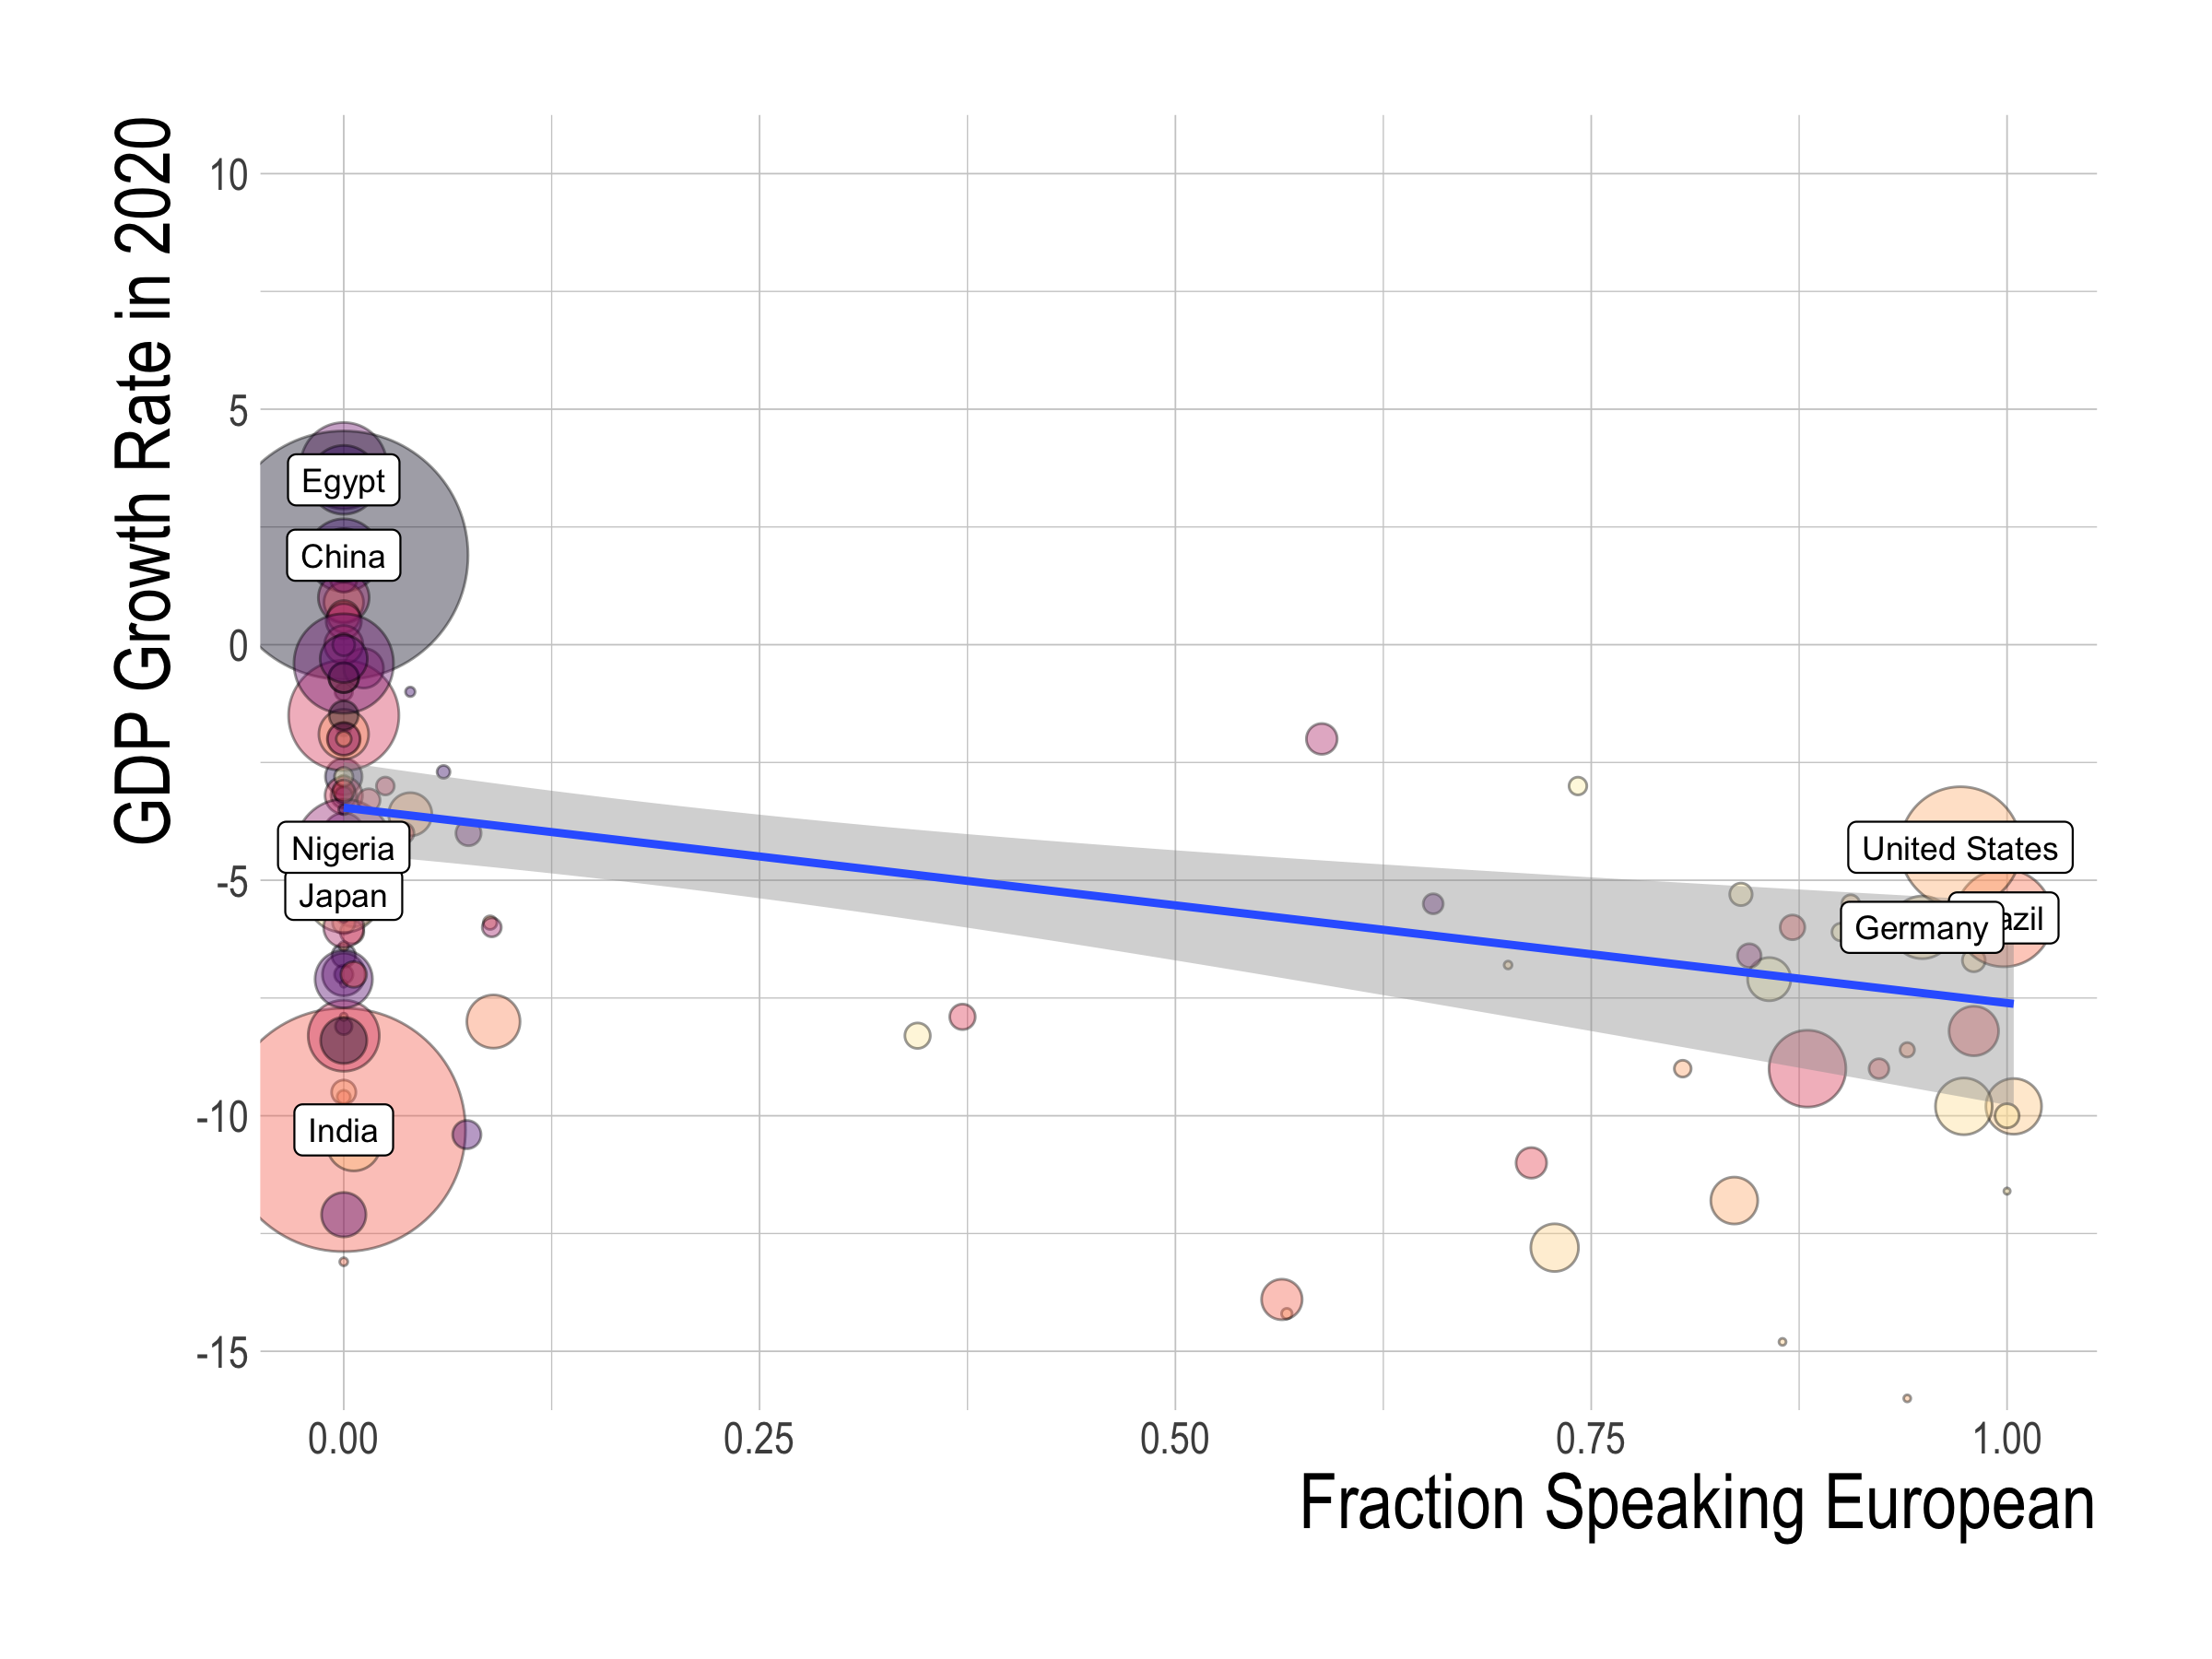
\includegraphics[width=5in]{plots/gdp_eurfrac_noControls_popWeighted_ols.png}}\hspace{1em}%
    \subcaptionbox{Total Covid-19-related Deaths Per Million\label{fig:reduced-deaths-eurfrac}}{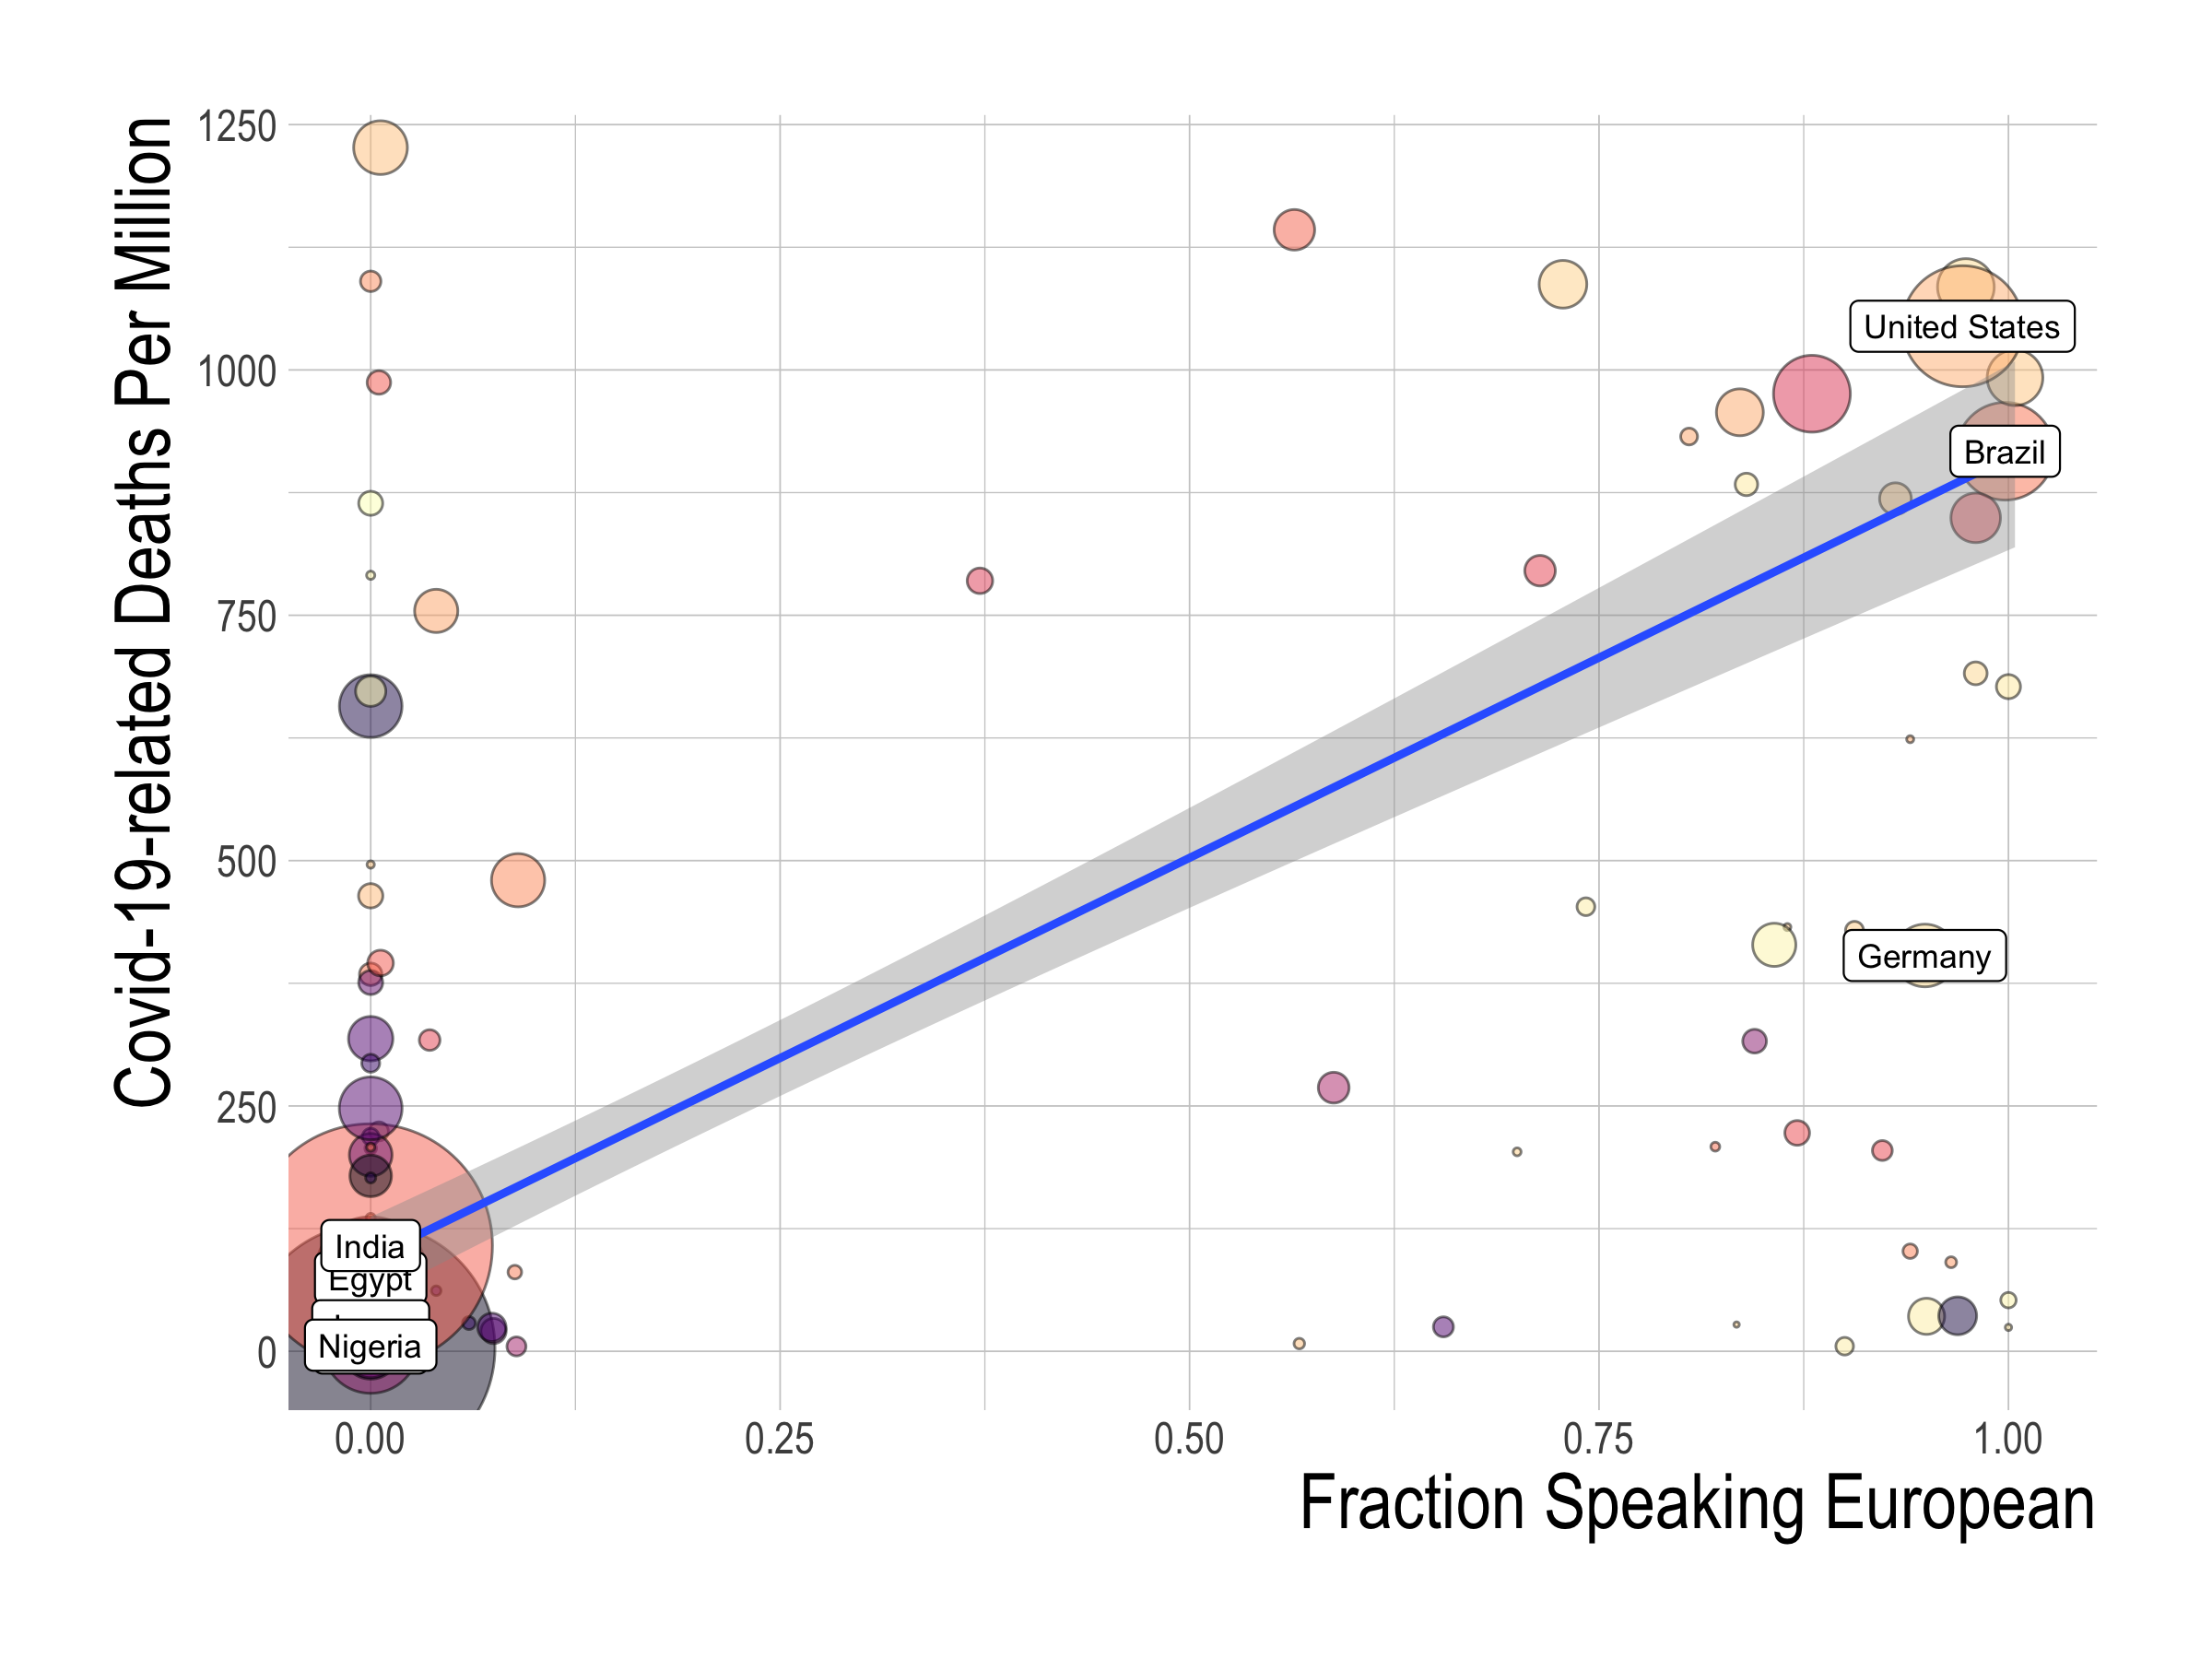
\includegraphics[width=5in]{plots/deaths_eurfrac_noControls_popWeighted_ols.png}}\hspace{1em}%
  
  \caption*{\textit{Notes:} The size of each observation point is proportional to the size of the population of each country. The colors vary depending on the level of the Democracy Index (Freedom House). The regression line corresponds to the reduced-form OLS regression without controls and weighted by population. The shaded area corresponds to the 95\% confidence interval.}
  
\end{figure}
% \begin{figure}[!htbp]
\centering
\caption{Reduced Form Relationship Between Covid-19-related Outcomes and Population Density in 1500}
\centering
\label{fig:reduced-form-lpd}
  \subcaptionbox{GDP Growth Rates in 2020 \label{fig:reduced-gdp-lpd}}{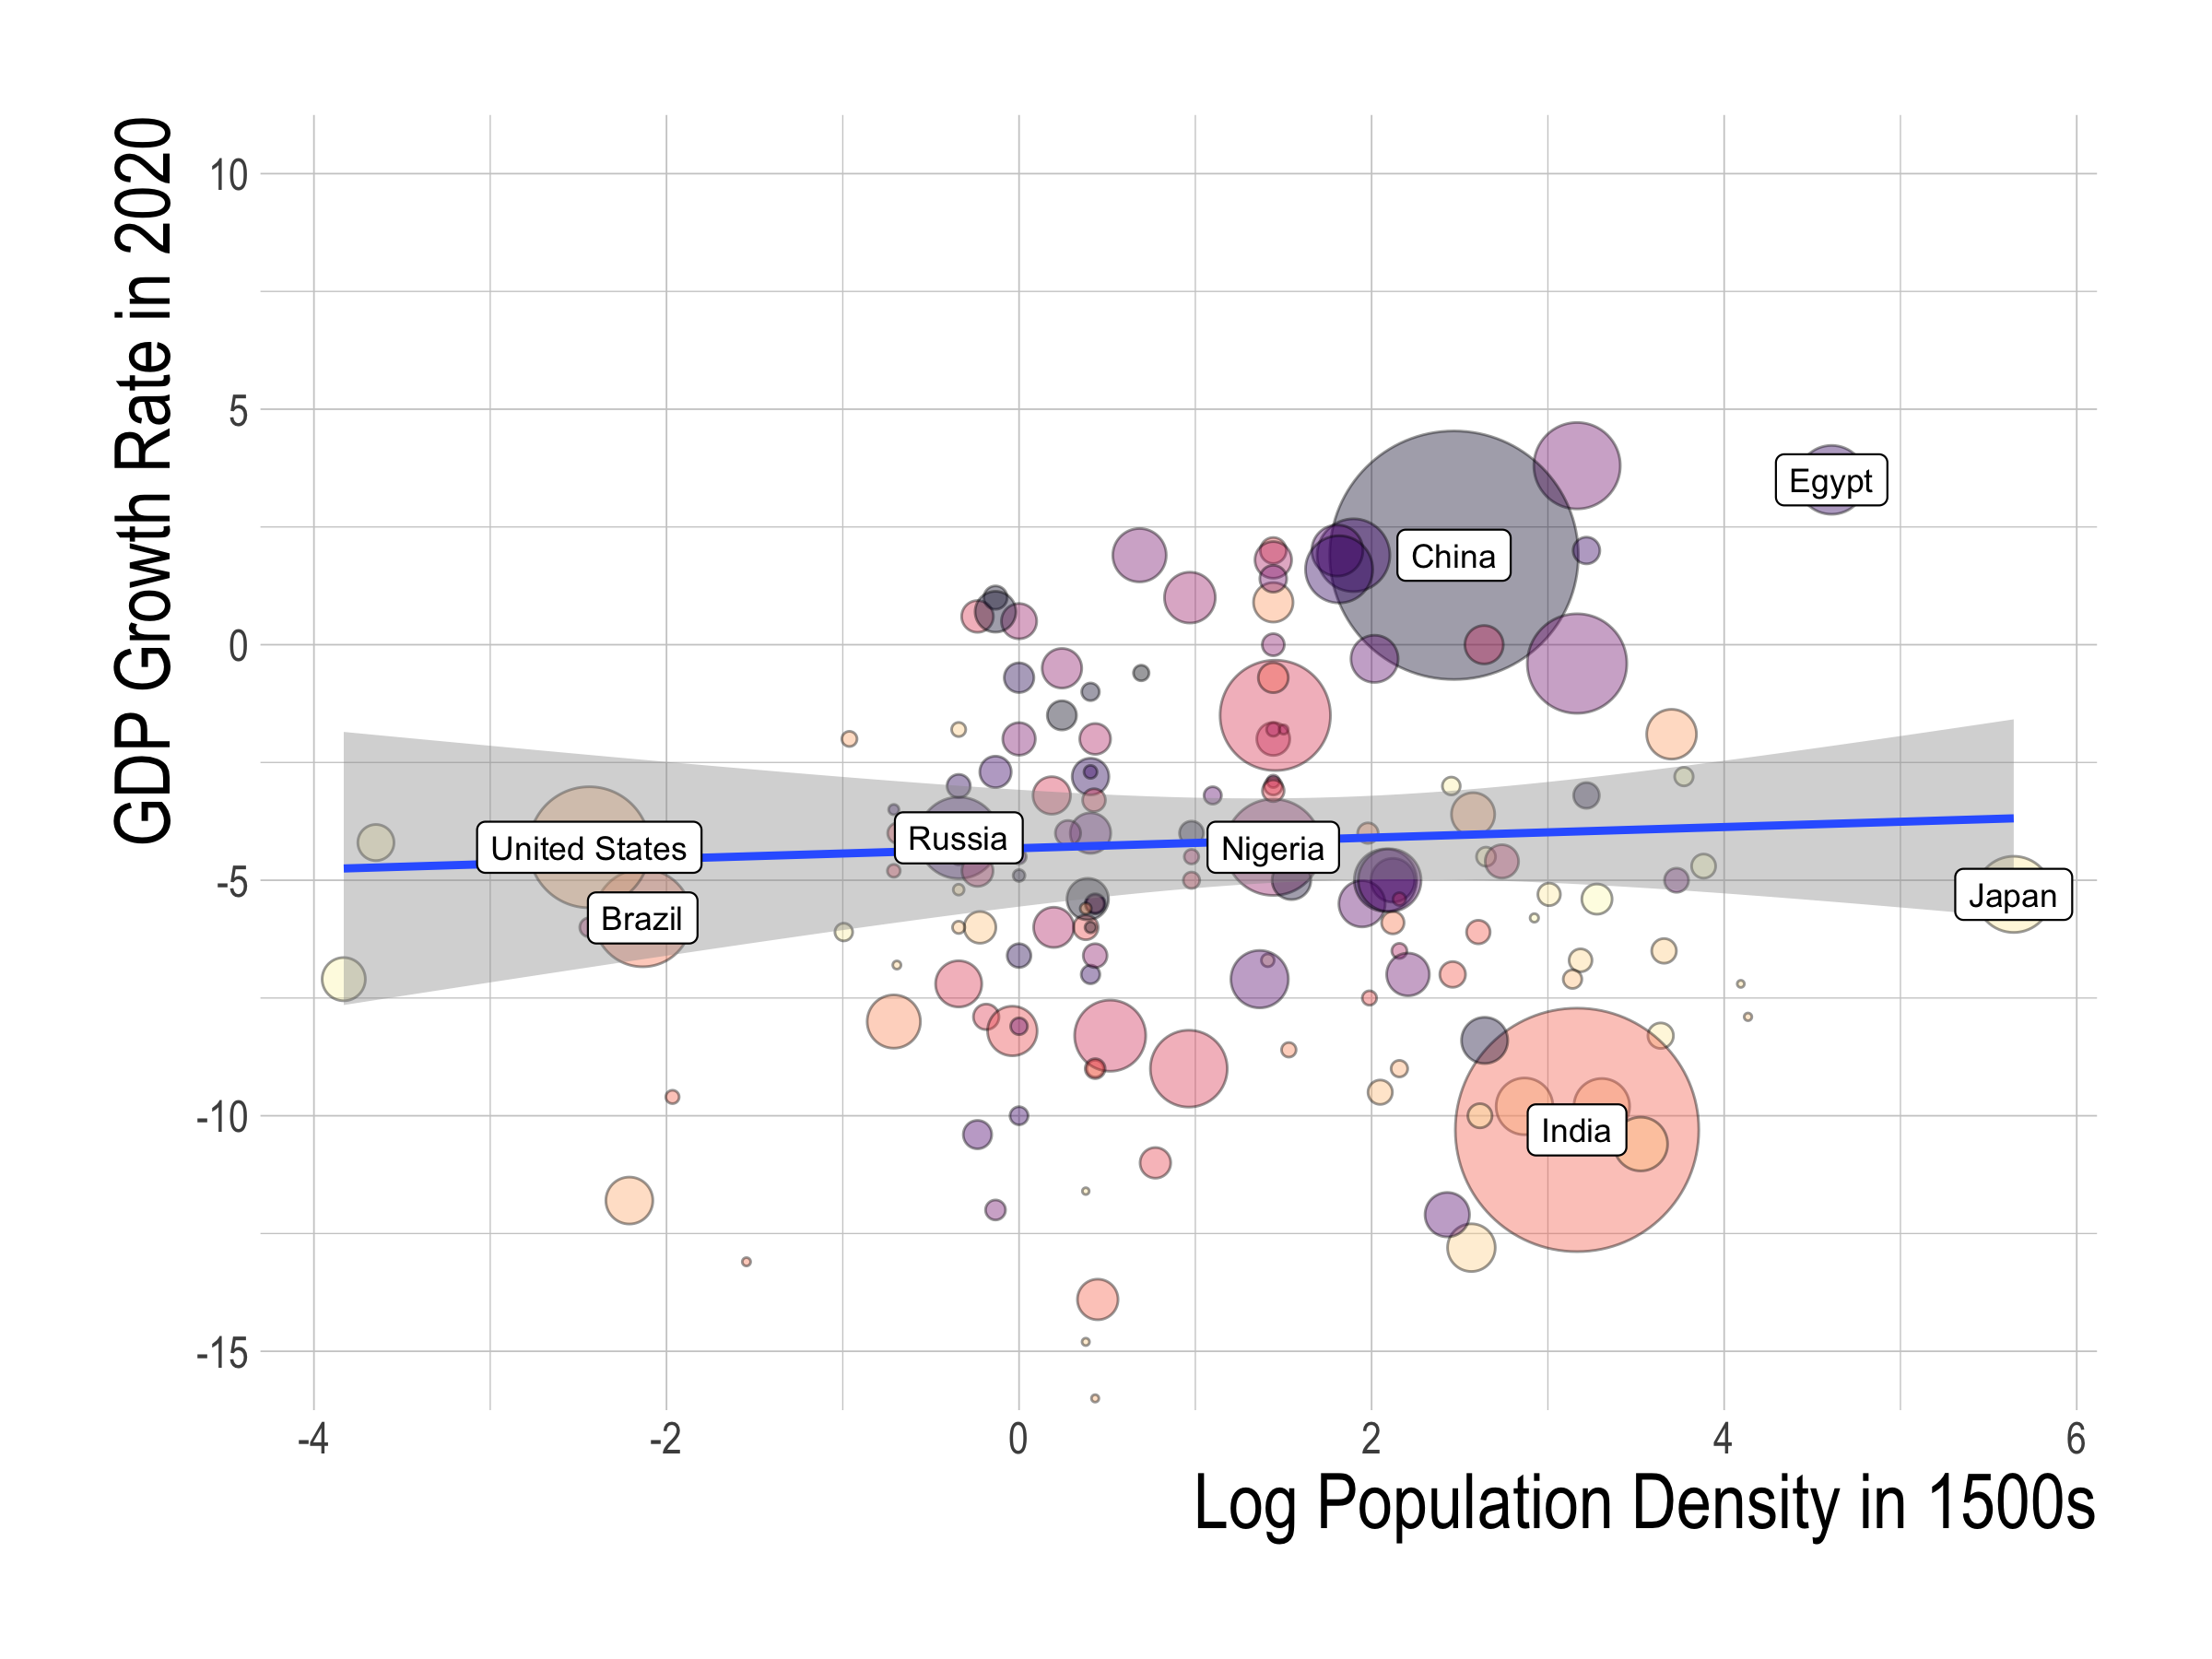
\includegraphics[width=5in]{plots/gdp_lpd1500s_noControls_popWeighted_ols.png}}
      \subcaptionbox{Total Covid-19-related Deaths Per Million\label{fig:reduced-deaths-lpd}}{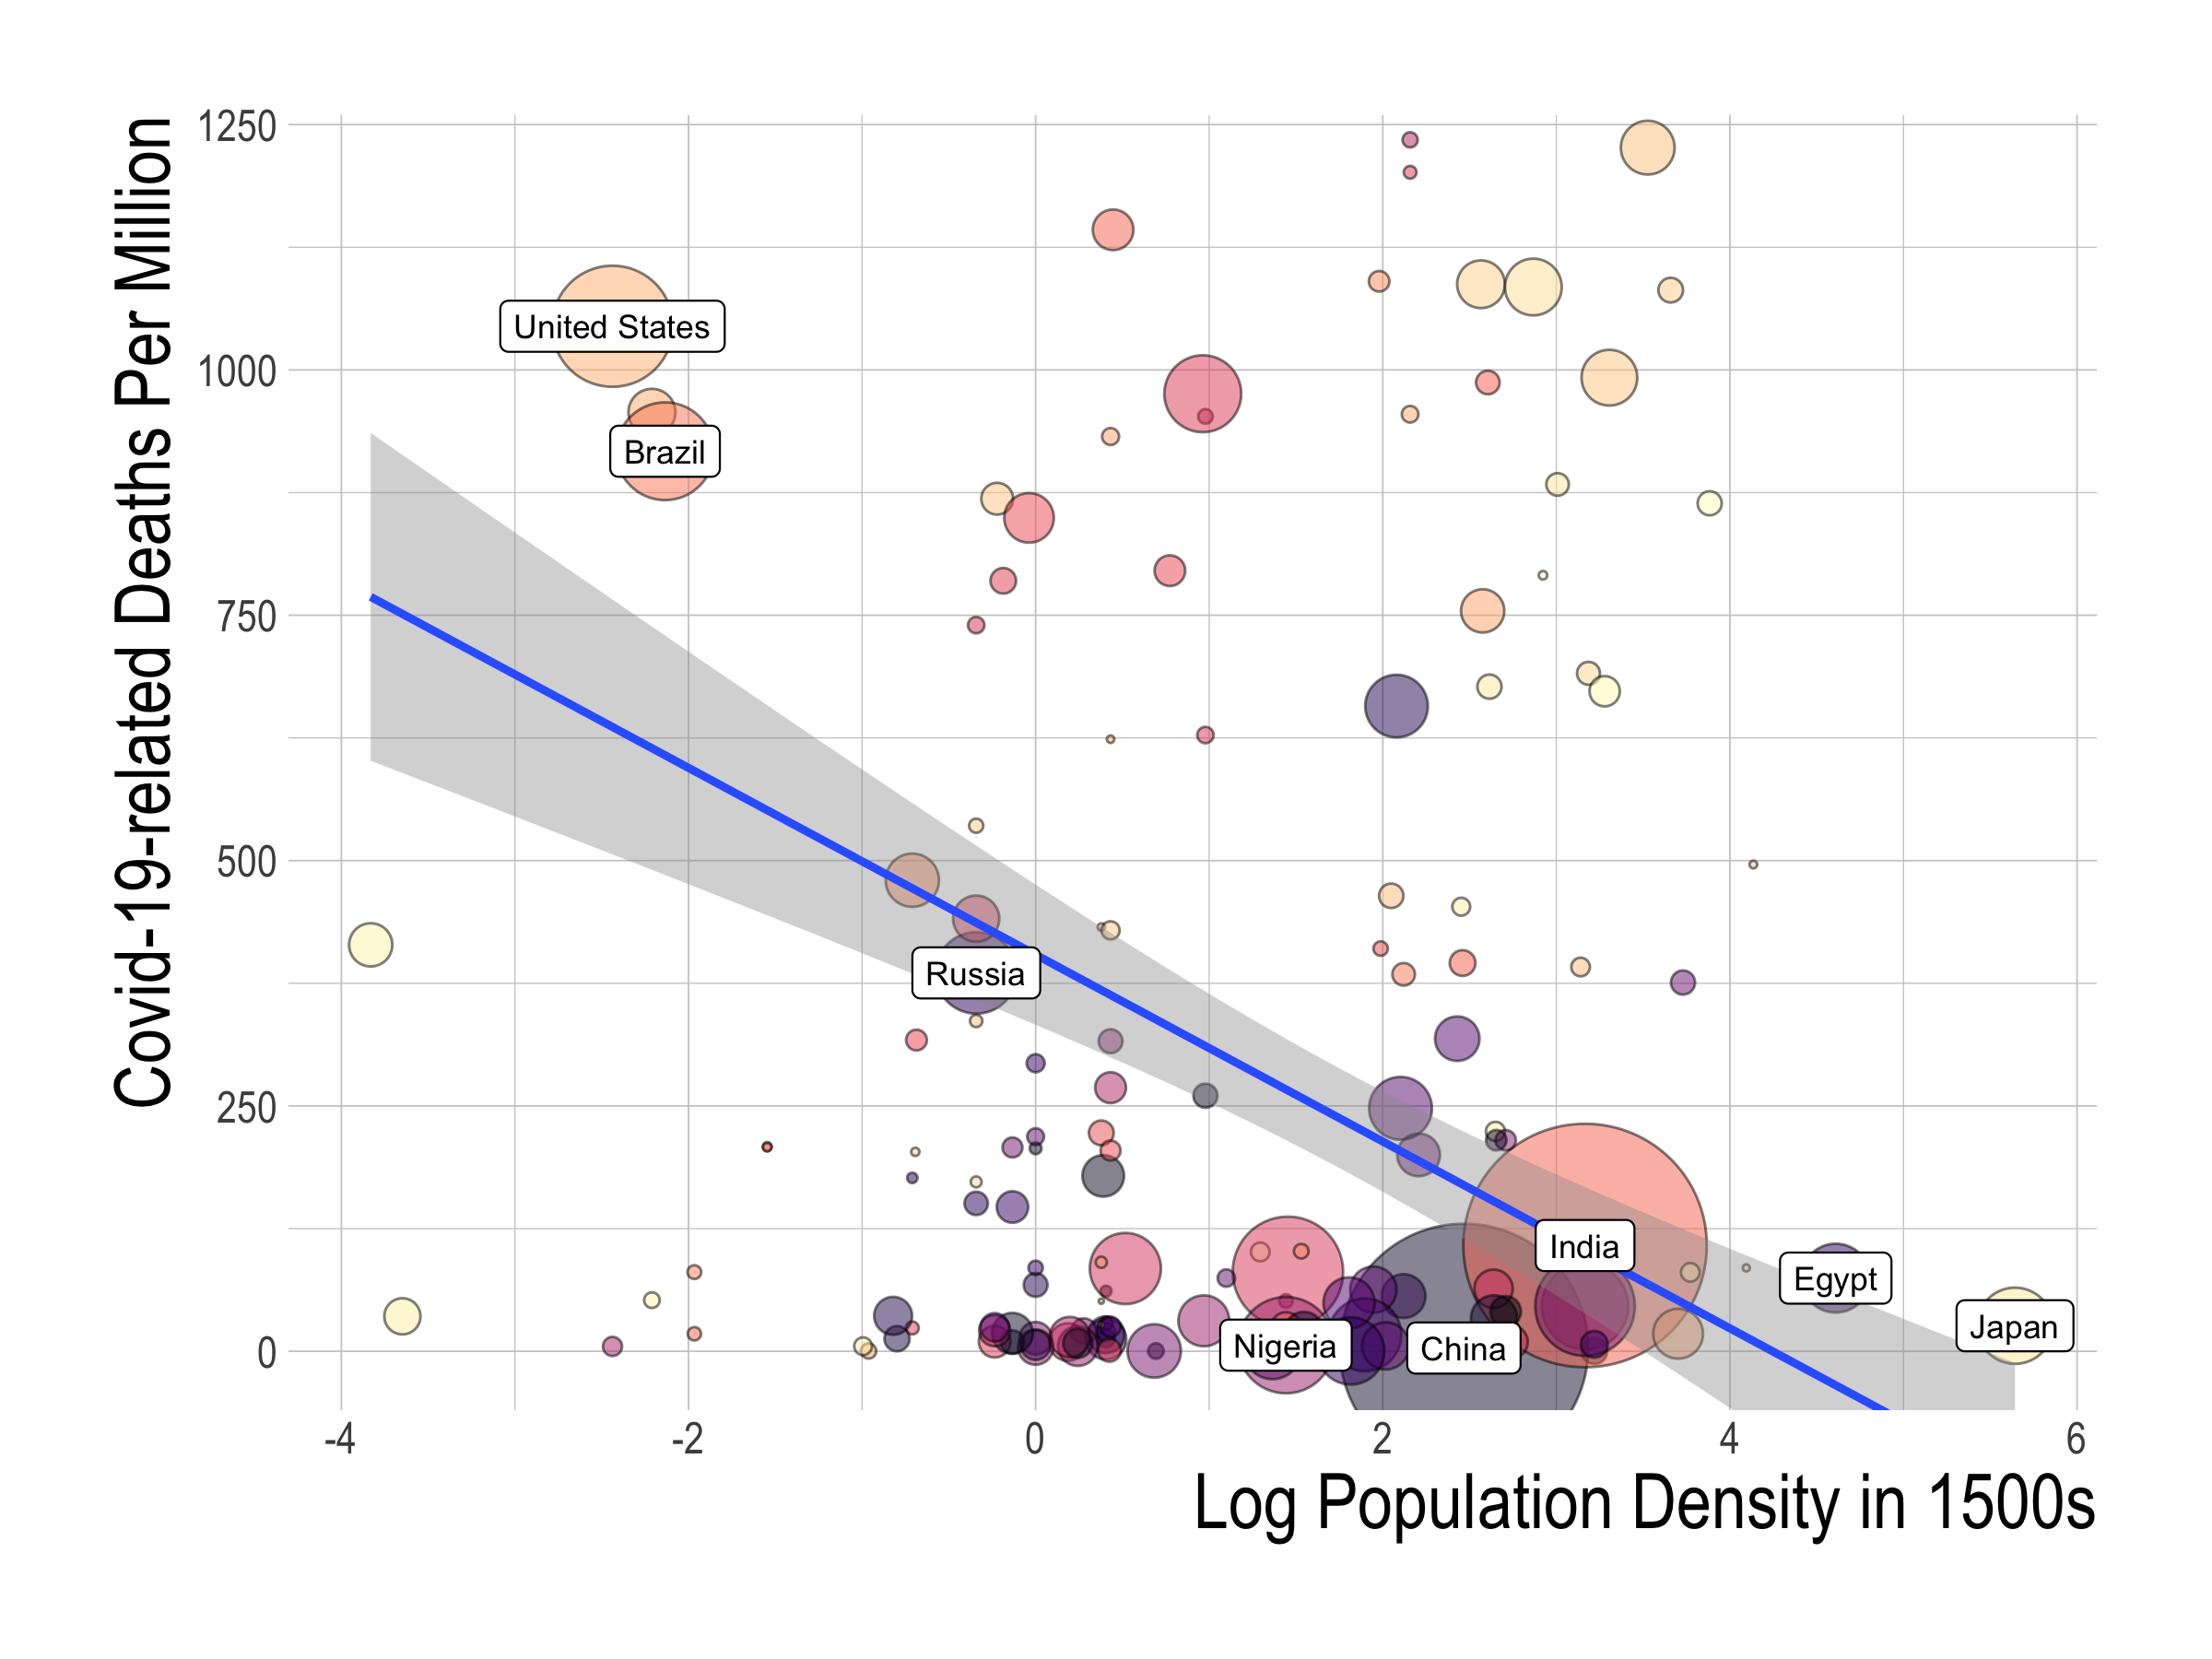
\includegraphics[width=5in]{plots/deaths_lpd1500s_noControls_popWeighted_ols.png}}
  \caption*{\textit{Notes:} The size of each observation point is proportional to the size of the population of each country. The colors vary depending on the level of the Democracy Index (Freedom House). The regression line corresponds to the reduced-form OLS regression without controls and weighted by population. The shaded area corresponds to the 95\% confidence interval.}
  
\end{figure}

% \newpage
% \setcounter{table}{0}
% \subsection{Use the Same Sample among Different IVs}
% 
\begin{table}[!htbp] 
  \caption{2SLS Regressions on GDP Growth Rates in 2020}
  \label{tab:2sls-gdp-restrict-sample} 
  \footnotesize
  \begin{threeparttable}
\begin{tabular}{@{\extracolsep{0pt}}lcccccccccc} 
\\[-1.8ex]\hline 
\hline \\[-1.8ex] 
 & \multicolumn{10}{c}{\textit{Dependent variable:}} \\ 
\cline{2-11} 
\\[-1.8ex] & \multicolumn{10}{c}{GDP Growth Rates in 2020} \\ 
\\[-1.8ex] & (1) & (2) & (3) & (4) & (5) & (6) & (7) & (8) & (9) & (10)\\ 
\hline \\[-1.8ex] 
  & \multicolumn{10}{c}{Panel A: Two-Stage Least Squares} \\
   Democracy Index & $-$4.4$^{***}$ & $-$3.8$^{***}$ & $-$2.6 & $-$3.2$^{***}$ & $-$4.6$^{***}$ & $-$3.6$^{***}$ & $-$2.5 & $-$4.8$^{***}$ & $-$1.3 & $-$2.5$^{**}$ \\ 
 (Freedom House) & (1.4) & (1.1) & (1.7) & (0.9) & (0.9) & (0.9) & (3.2) & (1.4) & (3.3) & (1.1) \\ 
 \hline \\[-1.8ex] 
   & \multicolumn{10}{c}{Panel B: First Stage for the Democracy Index (Freedom House)} \\
  Log European Settler Mortality & $-$0.4$^{**}$ & $-$0.5$^{***}$ &  &  &  &  &  &  &  &  \\ 
  & (0.2) & (0.2) &  &  &  &  &  &  &  &  \\ 
  Fraction Speaking English &  &  & 0.8$^{***}$ & 1.4$^{***}$ &  &  &  &  &  &  \\ 
  &  &  & (0.2) & (0.4) &  &  &  &  &  &  \\ 
  Fraction Speaking European &  &  & 1.0$^{**}$ & 0.9$^{***}$ &  &  &  &  &  &  \\ 
  &  &  & (0.4) & (0.3) &  &  &  &  &  &  \\ 
  Frankel-Romer Trade Share &  &  & 0.2 & $-$0.3 &  &  &  &  &  &  \\ 
  &  &  & (0.4) & (0.2) &  &  &  &  &  &  \\ 
  British Legal Origin &  &  &  &  & 1.7$^{***}$ & 2.5$^{***}$ &  &  &  &  \\ 
  &  &  &  &  & (0.2) & (0.2) &  &  &  &  \\ 
  French Legal Origin &  &  &  &  & 1.4$^{***}$ & 2.2$^{***}$ &  &  &  &  \\ 
  &  &  &  &  & (0.2) & (0.2) &  &  &  &  \\ 
  Bananas &  &  &  &  &  &  & $-$0.1 & $-$0.1 &  &  \\ 
  &  &  &  &  &  &  & (0.4) & (0.2) &  &  \\ 
  Coffee &  &  &  &  &  &  & 0.5 & 1.4$^{***}$ &  &  \\ 
  &  &  &  &  &  &  & (0.4) & (0.4) &  &  \\ 
  Maize &  &  &  &  &  &  & 1.4$^{*}$ & 2.1$^{***}$ &  &  \\ 
  &  &  &  &  &  &  & (0.8) & (0.8) &  &  \\ 
  Millet &  &  &  &  &  &  & $-$0.2 & 0.8$^{**}$ &  &  \\ 
  &  &  &  &  &  &  & (0.5) & (0.3) &  &  \\ 
  Rice &  &  &  &  &  &  & $-$0.6 & $-$2.6$^{***}$ &  &  \\ 
  &  &  &  &  &  &  & (0.6) & (1.0) &  &  \\ 
  Sugar &  &  &  &  &  &  & $-$0.7 & $-$0.6 &  &  \\ 
  &  &  &  &  &  &  & (0.7) & (0.6) &  &  \\ 
  Rubber &  &  &  &  &  &  & $-$0.5 & $-$1.3$^{***}$ &  &  \\ 
  &  &  &  &  &  &  & (0.6) & (0.4) &  &  \\ 
  Wheat &  &  &  &  &  &  & $-$0.1 & 0.001 &  &  \\ 
  &  &  &  &  &  &  & (0.4) & (0.3) &  &  \\ 
  Log Population Density in 1500s &  &  &  &  &  &  &  &  & $-$0.2 & $-$0.3$^{***}$ \\ 
  &  &  &  &  &  &  &  &  & (0.1) & (0.1) \\ 
R$^{2}$ & 0.2 & 0.6 & 0.3 & 0.7 & 0.6 & 0.8 & 0.1 & 0.7 & 0.1 & 0.6 \\ 
F Statistic & 19.0$^{***}$ & 12.7$^{***}$ & 11.0$^{***}$ & 16.8$^{***}$ & 50.5$^{***}$ & 28.9$^{***}$ & 1.0 & 9.6$^{***}$ & 11.0$^{***}$ & 13.1$^{***}$ \\ 

 \hline \\[-1.8ex] 
   & \multicolumn{10}{c}{Panel C: Ordinary Least Squares} \\
Democracy Index & $-$4.0$^{***}$ & $-$3.5$^{***}$ & $-$4.0$^{***}$ & $-$3.5$^{***}$ & $-$4.0$^{***}$ & $-$3.5$^{***}$ & $-$4.0$^{***}$ & $-$3.5$^{***}$ & $-$4.0$^{***}$ & $-$3.5$^{***}$ \\ 
 (Freedom House)  & (0.8) & (0.8) & (0.8) & (0.8) & (0.8) & (0.8) & (0.8) & (0.8) & (0.5) & (0.5) \\ 
R$^{2}$ & 0.5 & 0.6 & 0.5 & 0.6 & 0.5 & 0.6 & 0.5 & 0.6 & 0.5 & 0.6 \\ 
  \hline \\[-1.8ex] 
Weighting & Pop & Pop & Pop & Pop & Pop & Pop & Pop & Pop & Pop & Pop \\ 
Controls & \xmark & \cmark & \xmark & \cmark & \xmark & \cmark & \xmark & \cmark & \xmark & \cmark\\ 
N & 78 & 78 & 78 & 78 & 78 & 78 & 78 & 78 & 78 & 78 \\ 
\hline 
\hline \\[-1.8ex] 
  & \multicolumn{10}{r}{$^{*}$p$<$0.1; $^{**}$p$<$0.05; $^{***}$p$<$0.01} \\ 
\end{tabular} 
\begin{tablenotes} 
\item {\footnotesize {\textit{Notes:}  The Democracy Index (Freedom House) is the sum of the political rights and civil liberties scales from Freedom in the World 2020 by Freedom House and has been normalized by its standard deviation. Panel A reports the two-stage least squares estimates of the effect of democracy on GDP growth rates in 2020, using five different instrumental variable strategies. Panel B reports the corresponding first stage regressions. Panel C reports the coefficients from an OLS regression of GDP growth rates in 2020 against the Freedom House index. Columns (1), (3), (5), (7) and (9) have no controls, while columns (2), (4), (6), (8) and (10) have the following controls: absolute latitude, mean temperature, mean precipitation, population density, median age and diabetes prevalence. All regressions have been weighted by population. Robust standard errors are in parentheses. }}
\end{tablenotes}
\end{threeparttable}
\end{table} 


% 
\begin{table}[!htbp] \centering
  \caption{2SLS Regressions on Covid-19-related Deaths Per Million}
  \label{tab:2sls-deaths-restrict-sample} 
  \footnotesize
  \begin{threeparttable}
\begin{tabular}{@{\extracolsep{0pt}}lcccccccccc} 
\\[-1.8ex]\hline 
\hline \\[-1.8ex] 
 & \multicolumn{10}{c}{\textit{Dependent variable:}} \\ 
\cline{2-11} 
\\[-1.8ex] & \multicolumn{10}{c}{Covid-19-related Deaths Per Million} \\ 
\\[-1.8ex] & (1) & (2) & (3) & (4) & (5) & (6) & (7) & (8) & (9) & (10)\\ 
\hline \\[-1.8ex] 
  & \multicolumn{10}{c}{Panel A: Two-Stage Least Squares} \\
Democracy index & 428.1$^{***}$ & 394.7$^{***}$ & 566.4$^{**}$ & 475.6$^{***}$ & 145.5$^{**}$ & 368.9$^{***}$ & 443.9 & 263.8$^{***}$ & 678.0$^{*}$ & 532.9$^{***}$ \\ 
(Freedom House)  & (151.8) & (66.9) & (242.3) & (71.1) & (66.7) & (56.4) & (316.2) & (95.0) & (390.8) & (140.0) \\ 
\hline \\[-1.8ex] 
   & \multicolumn{10}{c}{Panel B: First Stage for the Democracy Index (Freedom House)} \\
  Log European Settler Mortality & $-$0.4$^{**}$ & $-$0.5$^{***}$ &  &  &  &  &  &  &  &  \\ 
  & (0.2) & (0.2) &  &  &  &  &  &  &  &  \\ 
  Fraction Speaking English &  &  & 0.8$^{***}$ & 1.4$^{***}$ &  &  &  &  &  &  \\ 
  &  &  & (0.2) & (0.4) &  &  &  &  &  &  \\ 
  Fraction Speaking European &  &  & 1.0$^{**}$ & 0.9$^{***}$ &  &  &  &  &  &  \\ 
  &  &  & (0.4) & (0.3) &  &  &  &  &  &  \\ 
  Frankel-Romer Trade Share &  &  & 0.2 & $-$0.3 &  &  &  &  &  &  \\ 
  &  &  & (0.4) & (0.2) &  &  &  &  &  &  \\ 
  British Legal Origin &  &  &  &  & 1.7$^{***}$ & 2.5$^{***}$ &  &  &  &  \\ 
  &  &  &  &  & (0.2) & (0.2) &  &  &  &  \\ 
  French Legal Origin &  &  &  &  & 1.4$^{***}$ & 2.2$^{***}$ &  &  &  &  \\ 
  &  &  &  &  & (0.2) & (0.2) &  &  &  &  \\ 
  Bananas &  &  &  &  &  &  & $-$0.1 & $-$0.1 &  &  \\ 
  &  &  &  &  &  &  & (0.4) & (0.2) &  &  \\ 
  Coffee &  &  &  &  &  &  & 0.5 & 1.4$^{***}$ &  &  \\ 
  &  &  &  &  &  &  & (0.4) & (0.4) &  &  \\ 
  Maize &  &  &  &  &  &  & 1.4$^{*}$ & 2.1$^{***}$ &  &  \\ 
  &  &  &  &  &  &  & (0.8) & (0.8) &  &  \\ 
  Millet &  &  &  &  &  &  & $-$0.2 & 0.8$^{**}$ &  &  \\ 
  &  &  &  &  &  &  & (0.5) & (0.3) &  &  \\ 
  Rice &  &  &  &  &  &  & $-$0.6 & $-$2.6$^{***}$ &  &  \\ 
  &  &  &  &  &  &  & (0.6) & (1.0) &  &  \\ 
  Sugarcane &  &  &  &  &  &  & $-$0.7 & $-$0.6 &  &  \\ 
  &  &  &  &  &  &  & (0.7) & (0.6) &  &  \\ 
  Rubber &  &  &  &  &  &  & $-$0.5 & $-$1.3$^{***}$ &  &  \\ 
  &  &  &  &  &  &  & (0.6) & (0.4) &  &  \\ 
  Wheat &  &  &  &  &  &  & $-$0.1 & 0.001 &  &  \\ 
  &  &  &  &  &  &  & (0.4) & (0.3) &  &  \\ 
  Log Population Density in 1500s &  &  &  &  &  &  &  &  & $-$0.2 & $-$0.3$^{***}$ \\ 
  &  &  &  &  &  &  &  &  & (0.1) & (0.1) \\ 
R$^{2}$ & 0.2 & 0.6 & 0.3 & 0.7 & 0.6 & 0.8 & 0.1 & 0.7 & 0.1 & 0.6 \\ 
F Statistic & 19.0$^{***}$ & 12.7$^{***}$ & 11.0$^{***}$ & 16.8$^{***}$ & 50.5$^{***}$& 28.9$^{***}$ & 1.0 & 9.6$^{***}$ & 11.0$^{***}$ & 13.1$^{***}$\\ 
% F Statistic & 20.2$^{***}$ (df = 1; 82) & 10.8$^{***}$ (df = 7; 76) & 11.5$^{***}$ (df = 3; 77) & 17.5$^{***}$ (df = 9; 71) & 48.2$^{***}$ (df = 2; 81) & 23.5$^{***}$ (df = 8; 75) & 1.1 (df = 8; 75) & 7.3$^{***}$ (df = 14; 69) & 11.3$^{***}$ (df = 1; 79) & 11.2$^{***}$ (df = 7; 73) \\ 
 
 \hline \\[-1.8ex] 
  & \multicolumn{10}{c}{Panel C: Ordinary Least Squares} \\
 Democracy Index (Freedom House) & 220.0$^{***}$ & 284.1$^{***}$ & 220.0$^{***}$ & 284.1$^{***}$ & 220.0$^{***}$ & 284.1$^{***}$ & 220.0$^{***}$ & 284.1$^{***}$ & 220.0$^{***}$ & 284.1$^{***}$ \\ 
 (Freedom House) & (78.9) & (65.5) & (78.9) & (65.5) & (78.9) & (65.5) & (78.9) & (65.5) & (34.5) & (37.5) \\
  \hline \\[-1.8ex] 
Weighting & Pop & Pop & Pop & Pop & Pop & Pop & Pop & Pop & Pop & Pop \\ 
Controls & \xmark & \cmark & \xmark & \cmark & \xmark & \cmark & \xmark & \cmark & \xmark & \cmark\\ 
N  & 78 & 78 & 78 & 78 & 78 & 78 & 78 & 78 & 78 & 78 \\ 
\hline 
\hline \\[-1.8ex] 
 & \multicolumn{10}{r}{$^{*}$p$<$0.1; $^{**}$p$<$0.05; $^{***}$p$<$0.01} \\ 
\end{tabular} 
\begin{tablenotes} 
\item {\footnotesize {\textit{Notes:} The Democracy Index (Freedom House) is the sum of the political rights and civil liberties scales from Freedom in the World 2020 by Freedom House and has been normalized by its standard deviation. Panel A reports the two-stage least squares estimates of the effect of democracy on Covid-19-related deaths per million, using five different instrumental variable strategies. Panel B reports the corresponding first stage regressions. Panel C reports the coefficients from an OLS regression of Covid-19-related deaths per million against the Freedom House index.  Columns (1), (3), (5), (7) and (9) have no controls, while columns (2), (4), (6), (8) and (10) have the following controls: absolute latitude, mean temperature, mean precipitation, population density, median age and diabetes prevalence. All regressions have been weighted by population.}}
\end{tablenotes}
\end{threeparttable}
\end{table} 


% \newpage
% \setcounter{table}{0}
% \subsection{Exclude US and China from Sample}
% 
\begin{table}[!htbp] 
  \caption{2SLS Regressions on GDP Growth Rates in 2020}
  \label{tab:2sls-gdp-exclude-US-China} 
  \footnotesize
  \begin{threeparttable}
\begin{tabular}{@{\extracolsep{0pt}}lcccccccccc} 
\\[-1.8ex]\hline 
\hline \\[-1.8ex] 
 & \multicolumn{10}{c}{\textit{Dependent variable:}} \\ 
\cline{2-11} 
\\[-1.8ex] & \multicolumn{10}{c}{GDP Growth Rates in 2020} \\ 
\\[-1.8ex] & (1) & (2) & (3) & (4) & (5) & (6) & (7) & (8) & (9) & (10)\\ 
\hline \\[-1.8ex] 

  & \multicolumn{10}{c}{Panel A: Two-Stage Least Squares} \\
 Democracy Index  & $-$6.4$^{***}$ & $-$7.3 & $-$5.2$^{***}$ & $-$5.6$^{***}$ & $-$3.5 & $-$4.9$^{**}$ & $-$6.1$^{***}$ & $-$7.0$^{***}$ & $-$3.0 & 5.2 \\ 
 (Freedom House) & (1.8) & (9.6) & (1.3) & (1.3) & (5.8) & (2.2) & (2.1) & (1.6) & (7.3) & (14.7) \\ 
 \hline \\[-1.8ex] 
 
 
   & \multicolumn{10}{c}{Panel B: First Stage for the Democracy Index (Freedom House)} \\
  Log European Settler Mortality & $-$0.2$^{***}$ & $-$0.1 &  &  &  &  &  &  &  &  \\ 
  & (0.1) & (0.1) &  &  &  &  &  &  &  &  \\ 
  Fraction Speaking English &  &  & 0.9$^{***}$ & 0.05 &  &  &  &  &  &  \\ 
  &  &  & (0.3) & (0.2) &  &  &  &  &  &  \\ 
  Fraction Speaking European &  &  & 0.7$^{***}$ & 0.3$^{*}$ &  &  &  &  &  &  \\ 
  &  &  & (0.3) & (0.2) &  &  &  &  &  &  \\ 
  Frankel-Romer Trade Share &  &  & $-$0.3$^{**}$ & $-$0.5$^{***}$ &  &  &  &  &  &  \\ 
  &  &  & (0.1) & (0.1) &  &  &  &  &  &  \\ 
  British Legal Origin &  &  &  &  & $-$0.01 & 0.9$^{***}$ &  &  &  &  \\ 
  &  &  &  &  & (0.5) & (0.3) &  &  &  &  \\ 
  French Legal Origin &  &  &  &  & $-$0.3 & 0.4 &  &  &  &  \\ 
  &  &  &  &  & (0.5) & (0.3) &  &  &  &  \\ 
  Bananas &  &  &  &  &  &  & 0.2 & 0.1 &  &  \\ 
  &  &  &  &  &  &  & (0.2) & (0.2) &  &  \\ 
  Coffee &  &  &  &  &  &  & 0.03 & 0.4 &  &  \\ 
  &  &  &  &  &  &  & (0.3) & (0.3) &  &  \\ 
  Maize &  &  &  &  &  &  & 0.5 & 0.2 &  &  \\ 
  &  &  &  &  &  &  & (0.5) & (0.4) &  &  \\ 
  Millet &  &  &  &  &  &  & $-$0.3 & $-$0.01 &  &  \\ 
  &  &  &  &  &  &  & (0.2) & (0.2) &  &  \\ 
  Rice &  &  &  &  &  &  & $-$0.4 & $-$0.3 &  &  \\ 
  &  &  &  &  &  &  & (0.4) & (0.3) &  &  \\ 
  Sugar &  &  &  &  &  &  & $-$0.4 & 0.1 &  &  \\ 
  &  &  &  &  &  &  & (0.4) & (0.3) &  &  \\ 
  Rubber &  &  &  &  &  &  & 0.5$^{*}$ & 0.2 &  &  \\ 
  &  &  &  &  &  &  & (0.3) & (0.2) &  &  \\ 
  Wheat &  &  &  &  &  &  & 0.6$^{**}$ & 0.5 &  &  \\ 
  &  &  &  &  &  &  & (0.2) & (0.4) &  &  \\ 
  Log Population Density in 1500s &  &  &  &  &  &  &  &  & 0.1 & 0.04 \\ 
  &  &  &  &  &  &  &  &  & (0.1) & (0.1) \\ 
R$^{2}$ & 0.1 & 0.3 & 0.3 & 0.6 & 0.03 & 0.4 & 0.2 & 0.4 & 0.02 & 0.3 \\ 
F Statistic & 13.1$^{***}$ & 4.7$^{***}$ & 15.3$^{***}$ & 22.2$^{***}$ & 2.0 & 11.5$^{***}$ & 3.4$^{***}$ & 8.3$^{***}$ & 2.4 & 9.6$^{***}$ \\

 \hline \\[-1.8ex] 
   & \multicolumn{10}{c}{Panel C: Ordinary Least Squares} \\
Democracy Index & $-$4.3$^{***}$ & $-$4.2$^{***}$ & $-$2.8$^{***}$ & $-$3.3$^{***}$ & $-$2.7$^{***}$ & $-$2.8$^{***}$ & $-$2.6$^{***}$ & $-$2.7$^{***}$ & $-$2.7$^{***}$ & $-$2.7$^{***}$ \\ 
 (Freedom House)  & (1.2) & (1.3) & (0.9) & (1.3) & (0.9) & (1.0) & (0.8) & (1.0) & (0.5) & (0.6) \\ 
R$^{2}$ & 0.3 & 0.5 & 0.2 & 0.4 & 0.2 & 0.3 & 0.2 & 0.3 & 0.2 & 0.3 \\ 
  \hline \\[-1.8ex] 
Weighting & Pop & Pop & Pop & Pop & Pop & Pop & Pop & Pop & Pop & Pop \\ 
Controls & \xmark & \cmark & \xmark & \cmark & \xmark & \cmark & \xmark & \cmark & \xmark & \cmark\\ 
N & 82 & 82 & 127 & 127 & 151 & 151 & 159 & 159 & 151 & 151 \\ 
\hline 
\hline \\[-1.8ex] 
  & \multicolumn{10}{r}{$^{*}$p$<$0.1; $^{**}$p$<$0.05; $^{***}$p$<$0.01} \\ 
\end{tabular} 
\begin{tablenotes} 
\item {\footnotesize {\textit{Notes:}  The Democracy Index (Freedom House) is the sum of the political rights and civil liberties scales from Freedom in the World 2020 by Freedom House and has been normalized by its standard deviation. Panel A reports the two-stage least squares estimates of the effect of democracy on GDP growth rates in 2020, using five different instrumental variable strategies. Panel B reports the corresponding first stage regressions. Panel C reports the coefficients from an OLS regression of GDP growth rates in 2020 against the Freedom House index. Columns (1), (3), (5), (7) and (9) have no controls, while columns (2), (4), (6), (8) and (10) have the following controls: absolute latitude, mean temperature, mean precipitation, population density, median age and diabetes prevalence. All regressions have been weighted by population. Robust standard errors are in parentheses. }}
\end{tablenotes}
\end{threeparttable}
\end{table} 


% 
\begin{table}[!htbp] \centering
  \caption{2SLS Regressions on Covid-19-related Deaths Per Million}
  \label{tab:2sls-deaths-exclude-US-China} 
  \footnotesize
  \begin{threeparttable}
\begin{tabular}{@{\extracolsep{0pt}}lcccccccccc} 
\\[-1.8ex]\hline 
\hline \\[-1.8ex] 
 & \multicolumn{10}{c}{\textit{Dependent variable:}} \\ 
\cline{2-11} 
\\[-1.8ex] & \multicolumn{10}{c}{Covid-19-related Deaths Per Million} \\ 
\\[-1.8ex] & (1) & (2) & (3) & (4) & (5) & (6) & (7) & (8) & (9) & (10)\\ 
\hline \\[-1.8ex] 
  & \multicolumn{10}{c}{Panel A: Two-Stage Least Squares} \\
Democracy Index& 459.8$^{**}$ & 769.0 & 435.2$^{***}$ & 172.9 & $-$900.7 & $-$54.0 & 246.4 & 108.3 & $-$912.1 & $-$1,605.3 \\ 
 (Freedom House)   & (179.9) & (1,355.1) & (161.1) & (164.5) & (977.6) & (160.6) & (224.3) & (133.3) & (1,540.1) & (2,456.5) \\ 
\hline \\[-1.8ex] 
   & \multicolumn{10}{c}{Panel B: First Stage for the Democracy Index (Freedom House)} \\
  Log European Settler Mortality & $-$0.2$^{***}$ & $-$0.1 &  &  &  &  &  &  &  &  \\ 
  & (0.1) & (0.1) &  &  &  &  &  &  &  &  \\ 
  Fraction Speaking English &  &  & 0.9$^{***}$ & 0.05 &  &  &  &  &  &  \\ 
  &  &  & (0.3) & (0.2) &  &  &  &  &  &  \\ 
  Fraction Speaking European &  &  & 0.7$^{***}$ & 0.3$^{*}$ &  &  &  &  &  &  \\ 
  &  &  & (0.3) & (0.2) &  &  &  &  &  &  \\ 
  Frankel-Romer Trade Share &  &  & $-$0.3$^{**}$ & $-$0.5$^{***}$ &  &  &  &  &  &  \\ 
  &  &  & (0.1) & (0.1) &  &  &  &  &  &  \\ 
  British Legal Origin &  &  &  &  & $-$0.01 & 0.9$^{***}$ &  &  &  &  \\ 
  &  &  &  &  & (0.5) & (0.3) &  &  &  &  \\ 
  French Legal Origin &  &  &  &  & $-$0.3 & 0.4 &  &  &  &  \\ 
  &  &  &  &  & (0.5) & (0.3) &  &  &  &  \\ 
  Bananas &  &  &  &  &  &  & 0.2 & 0.1 &  &  \\ 
  &  &  &  &  &  &  & (0.2) & (0.2) &  &  \\ 
  Coffee &  &  &  &  &  &  & 0.03 & 0.4 &  &  \\ 
  &  &  &  &  &  &  & (0.3) & (0.3) &  &  \\ 
  Maize &  &  &  &  &  &  & 0.5 & 0.2 &  &  \\ 
  &  &  &  &  &  &  & (0.5) & (0.4) &  &  \\ 
  Millet &  &  &  &  &  &  & $-$0.3 & $-$0.01 &  &  \\ 
  &  &  &  &  &  &  & (0.2) & (0.2) &  &  \\ 
  Rice &  &  &  &  &  &  & $-$0.4 & $-$0.3 &  &  \\ 
  &  &  &  &  &  &  & (0.4) & (0.3) &  &  \\ 
  Sugarcane &  &  &  &  &  &  & $-$0.4 & 0.1 &  &  \\ 
  &  &  &  &  &  &  & (0.4) & (0.3) &  &  \\ 
  Rubber &  &  &  &  &  &  & 0.5$^{*}$ & 0.2 &  &  \\ 
  &  &  &  &  &  &  & (0.3) & (0.2) &  &  \\ 
  Wheat &  &  &  &  &  &  & 0.6$^{**}$ & 0.5 &  &  \\ 
  &  &  &  &  &  &  & (0.2) & (0.4) &  &  \\ 
  Log Population Density in 1500s &  &  &  &  &  &  &  &  & 0.1 & 0.04 \\ 
  &  &  &  &  &  &  &  &  & (0.1) & (0.1) \\ 
R$^{2}$ & 0.1 & 0.3 & 0.3 & 0.6 & 0.03 & 0.4 & 0.2 & 0.4 & 0.02 & 0.3 \\ 
F Statistic & 13.1$^{***}$ & 4.7$^{***}$ & 15.3$^{***}$ & 22.2$^{***}$ & 2.0 & 11.5$^{***}$ & 3.4$^{***}$ & 8.3$^{***}$ & 2.4 & 9.6$^{***}$ \\ 

 \hline \\[-1.8ex] 
  & \multicolumn{10}{c}{Panel C: Ordinary Least Squares} \\
Democracy Index & 222.0$^{***}$ & 130.5$^{**}$ & 186.1$^{***}$ & 69.5 & 168.1$^{***}$ & 105.8$^{*}$ & 166.4$^{***}$ & 101.3$^{*}$ & 168.2$^{***}$ & 105.8$^{***}$ \\ 
 (Freedom House)  & (80.0) & (63.8) & (64.3) & (70.1) & (64.6) & (54.6) & (60.8) & (52.6) & (32.2) & (33.9) \\
 R$^{2}$ & 0.2 & 0.4 & 0.2 & 0.4 & 0.2 & 0.4 & 0.2 & 0.4 & 0.2 & 0.4 \\ 
\hline \\[-1.8ex]
Weighting & Pop & Pop & Pop & Pop & Pop & Pop & Pop & Pop & Pop & Pop \\ 
Controls & \xmark & \cmark & \xmark & \cmark & \xmark & \cmark & \xmark & \cmark & \xmark & \cmark\\ 
N & 82 & 82 & 127 & 127 & 151 & 151 & 159 & 159 & 151 & 151 \\ 
\hline 
\hline \\[-1.8ex] 
 & \multicolumn{10}{r}{$^{*}$p$<$0.1; $^{**}$p$<$0.05; $^{***}$p$<$0.01} \\ 
\end{tabular} 
\begin{tablenotes} 
\item {\footnotesize {\textit{Notes:} The Democracy Index (Freedom House) is the sum of the political rights and civil liberties scales from Freedom in the World 2020 by Freedom House and has been normalized by its standard deviation. Panel A reports the two-stage least squares estimates of the effect of democracy on Covid-19-related deaths per million, using five different instrumental variable strategies. Panel B reports the corresponding first stage regressions. Panel C reports the coefficients from an OLS regression of Covid-19-related deaths per million against the Freedom House index.  Columns (1), (3), (5), (7) and (9) have no controls, while columns (2), (4), (6), (8) and (10) have the following controls: absolute latitude, mean temperature, mean precipitation, population density, median age and diabetes prevalence. All regressions have been weighted by population.}}
\end{tablenotes}
\end{threeparttable}
\end{table} 




% \newpage
% \setcounter{table}{0}
% \subsection{Include Continent Dummies}
% 
\begin{table}[!htbp] \centering
  \caption{2SLS Regressions on GDP Growth Rates in 2020}
  \label{tab:2sls-gdp-continent} 
  \footnotesize
  \begin{threeparttable}
\begin{tabular}{@{\extracolsep{0pt}}lcccccccccc} 
\\[-1.8ex]\hline 
\hline \\[-1.8ex] 
 & \multicolumn{10}{c}{\textit{Dependent variable:}} \\ 
\cline{2-11} 
\\[-1.8ex] & \multicolumn{10}{c}{Covid-19-related Deaths Per Million} \\ 
\\[-1.8ex] & (1) & (2) & (3) & (4) & (5) & (6) & (7) & (8) & (9) & (10)\\ 
\hline \\[-1.8ex] 
  & \multicolumn{10}{c}{Panel A: Two-Stage Least Squares} \\
Democracy Index & $-$5.2$^{***}$ & $-$2.2 & $-$2.4 & $-$2.9$^{*}$ & $-$5.4$^{***}$ & $-$3.7$^{***}$ & $-$1.8 & $-$5.1$^{**}$ & $-$4.3 & $-$0.7 \\ 
(Freedom House)   & (2.0) & (2.1) & (3.7) & (1.6) & (0.9) & (1.0) & (2.8) & (2.1) & (2.8) & (4.2) \\ 
\hline \\[-1.8ex] 
   & \multicolumn{10}{c}{Panel B: First Stage for the Democracy Index (Freedom House)} \\
  Log European Settler Mortality & $-$0.3 & $-$0.3$^{**}$ &  &  &  &  &  &  &  &  \\ 
  & (0.3) & (0.1) &  &  &  &  &  &  &  &  \\ 
  Fraction Speaking English &  &  & 0.9$^{**}$ & 1.0$^{*}$ &  &  &  &  &  &  \\ 
  &  &  & (0.4) & (0.5) &  &  &  &  &  &  \\ 
  Fraction Speaking European &  &  & 0.2 & $-$0.1 &  &  &  &  &  &  \\ 
  &  &  & (0.2) & (0.3) &  &  &  &  &  &  \\ 
  Frankel-Romer Trade Share &  &  & 0.2 & $-$0.3 &  &  &  &  &  &  \\ 
  &  &  & (0.4) & (0.2) &  &  &  &  &  &  \\ 
  British Legal Origin &  &  &  &  & 1.4$^{***}$ & 1.3$^{***}$ &  &  &  &  \\ 
  &  &  &  &  & (0.4) & (0.3) &  &  &  &  \\ 
  French Legal Origin &  &  &  &  & 0.9$^{**}$ & 0.6$^{**}$ &  &  &  &  \\ 
  &  &  &  &  & (0.3) & (0.3) &  &  &  &  \\ 
  Bananas &  &  &  &  &  &  & $-$0.01 & 0.2 &  &  \\ 
  &  &  &  &  &  &  & (0.2) & (0.2) &  &  \\ 
  Coffee &  &  &  &  &  &  & $-$0.1 & 0.5 &  &  \\ 
  &  &  &  &  &  &  & (0.4) & (0.5) &  &  \\ 
  Maize &  &  &  &  &  &  & 0.9 & $-$0.1 &  &  \\ 
  &  &  &  &  &  &  & (0.7) & (0.4) &  &  \\ 
  Millet &  &  &  &  &  &  & $-$0.2 & 0.4 &  &  \\ 
  &  &  &  &  &  &  & (0.3) & (0.3) &  &  \\ 
  Rice &  &  &  &  &  &  & $-$0.03 & $-$0.4 &  &  \\ 
  &  &  &  &  &  &  & (0.3) & (0.4) &  &  \\ 
  Sugarcane &  &  &  &  &  &  & 0.2 & $-$0.2 &  &  \\ 
  &  &  &  &  &  &  & (0.3) & (0.3) &  &  \\ 
  Rubber &  &  &  &  &  &  & $-$0.01 & $-$0.5 &  &  \\ 
  &  &  &  &  &  &  & (0.3) & (0.3) &  &  \\ 
  Wheat &  &  &  &  &  &  & $-$0.1 & 0.3 &  &  \\ 
  &  &  &  &  &  &  & (0.5) & (0.4) &  &  \\ 
  Log Population Density in 1500s &  &  &  &  &  &  &  &  & 0.2 & 0.1 \\ 
  &  &  &  &  &  &  &  &  & (0.1) & (0.1) \\ 
R$^{2}$ & 0.3 & 0.6 & 0.3 & 0.7 & 0.5 & 0.7 & 0.3 & 0.6 & 0.3 & 0.6 \\ 
F Statistic & 6.4$^{***}$ & 10.7$^{***}$ & 7.8$^{***}$ & 15.7$^{***}$ & 23.7$^{***}$ & 20.7$^{***}$ & 4.1$^{***}$ & 11.6$^{***}$ & 8.8$^{***}$ & 15.4$^{***}$ \\ 
 \hline \\[-1.8ex] 
  & \multicolumn{10}{c}{Panel C: Ordinary Least Squares} \\
 Democracy Index & $-$4.3$^{***}$ & $-$3.4$^{***}$ & $-$3.7$^{***}$ & $-$3.0$^{***}$ & $-$3.4$^{***}$ & $-$2.9$^{***}$ & $-$3.3$^{***}$ & $-$2.8$^{***}$ & $-$3.4$^{***}$ & $-$2.9$^{***}$ \\ 
 (Freedom House) & (1.1) & (1.0) & (1.2) & (0.9) & (1.1) & (0.8) & (1.1) & (0.8) & (0.4) & (0.5) \\ 
R$^{2}$ & 0.6 & 0.7 & 0.5 & 0.6 & 0.4 & 0.5 & 0.4 & 0.5 & 0.4 & 0.5 \\ 
  \hline \\[-1.8ex] 

Weighting & Pop & Pop & Pop & Pop & Pop & Pop & Pop & Pop & Pop & Pop \\ 
Controls & \xmark & \cmark & \xmark & \cmark & \xmark & \cmark & \xmark & \cmark & \xmark & \cmark\\ 
N & 84 & 84 & 129 & 129 & 153 & 153 & 161 & 161 & 153 & 153 \\ 
\hline 
\hline \\[-1.8ex] 
 & \multicolumn{10}{r}{$^{*}$p$<$0.1; $^{**}$p$<$0.05; $^{***}$p$<$0.01} \\ 
\end{tabular} 
\begin{tablenotes} 
\item {\footnotesize {\textit{Notes:} The Democracy Index (Freedom House) is the sum of the political rights and civil liberties scales from Freedom in the World 2020 by Freedom House and has been normalized by its standard deviation. Panel A reports the two-stage least squares estimates of the effect of democracy on Covid-19-related deaths per million, using five different instrumental variable strategies. Panel B reports the corresponding first stage regressions. Panel C reports the coefficients from an OLS regression of Covid-19-related deaths per million against the Freedom House index.  Columns (1), (3), (5), (7) and (9) have no controls, while columns (2), (4), (6), (8) and (10) have the following controls: absolute latitude, mean temperature, mean precipitation, population density, median age and diabetes prevalence. All regressions have been weighted by population.}}
\end{tablenotes}
\end{threeparttable}
\end{table} 
% \end{adjustbox}
%}

%\end{adjustbox}

%\end{landscape}


% 
\begin{table}[!htbp] \centering
  \caption{2SLS Regressions on Covid-19-related Deaths Per Million}
  \label{tab:2sls-deaths-continent} 
  \footnotesize
  \begin{threeparttable}
\begin{tabular}{@{\extracolsep{0pt}}lcccccccccc} 
\\[-1.8ex]\hline 
\hline \\[-1.8ex] 
 & \multicolumn{10}{c}{\textit{Dependent variable:}} \\ 
\cline{2-11} 
\\[-1.8ex] & \multicolumn{10}{c}{Covid-19-related Deaths Per Million} \\ 
\\[-1.8ex] & (1) & (2) & (3) & (4) & (5) & (6) & (7) & (8) & (9) & (10)\\ 
\hline \\[-1.8ex] 
  & \multicolumn{10}{c}{Panel A: Two-Stage Least Squares} \\
Democracy Index & 206.5 & 182.3$^{**}$ & 166.7 & 213.6 & 95.2$^{***}$ & 126.9$^{*}$ & 73.2 & 107.0 & 81.7 & $-$55.5 \\ 
(Freedom House)  & (141.5) & (74.0) & (160.2) & (146.2) & (35.0) & (65.6) & (135.5) & (75.8) & (100.9) & (194.7) \\ 
\hline \\[-1.8ex] 
   & \multicolumn{10}{c}{Panel B: First Stage for the Democracy Index (Freedom House)} \\
  Log European Settler Mortality & $-$0.3 & $-$0.3$^{**}$ &  &  &  &  &  &  &  &  \\ 
  & (0.3) & (0.1) &  &  &  &  &  &  &  &  \\ 
  Fraction Speaking English &  &  & 0.9$^{**}$ & 1.0$^{*}$ &  &  &  &  &  &  \\ 
  &  &  & (0.4) & (0.5) &  &  &  &  &  &  \\ 
  Fraction Speaking European &  &  & 0.2 & $-$0.1 &  &  &  &  &  &  \\ 
  &  &  & (0.2) & (0.3) &  &  &  &  &  &  \\ 
  Frankel-Romer Trade Share &  &  & 0.2 & $-$0.3 &  &  &  &  &  &  \\ 
  &  &  & (0.4) & (0.2) &  &  &  &  &  &  \\ 
  British Legal Origin &  &  &  &  & 1.4$^{***}$ & 1.3$^{***}$ &  &  &  &  \\ 
  &  &  &  &  & (0.4) & (0.3) &  &  &  &  \\ 
  French Legal Origin &  &  &  &  & 0.9$^{**}$ & 0.6$^{**}$ &  &  &  &  \\ 
  &  &  &  &  & (0.3) & (0.3) &  &  &  &  \\ 
  Bananas &  &  &  &  &  &  & $-$0.01 & 0.2 &  &  \\ 
  &  &  &  &  &  &  & (0.2) & (0.2) &  &  \\ 
  Coffee &  &  &  &  &  &  & $-$0.1 & 0.5 &  &  \\ 
  &  &  &  &  &  &  & (0.4) & (0.5) &  &  \\ 
  Maize &  &  &  &  &  &  & 0.9 & $-$0.1 &  &  \\ 
  &  &  &  &  &  &  & (0.7) & (0.4) &  &  \\ 
  Millet &  &  &  &  &  &  & $-$0.2 & 0.4 &  &  \\ 
  &  &  &  &  &  &  & (0.3) & (0.3) &  &  \\ 
  Rice &  &  &  &  &  &  & $-$0.03 & $-$0.4 &  &  \\ 
  &  &  &  &  &  &  & (0.3) & (0.4) &  &  \\ 
  Sugarcane &  &  &  &  &  &  & 0.2 & $-$0.2 &  &  \\ 
  &  &  &  &  &  &  & (0.3) & (0.3) &  &  \\ 
  Rubber &  &  &  &  &  &  & $-$0.01 & $-$0.5 &  &  \\ 
  &  &  &  &  &  &  & (0.3) & (0.3) &  &  \\ 
  Wheat &  &  &  &  &  &  & $-$0.1 & 0.3 &  &  \\ 
  &  &  &  &  &  &  & (0.5) & (0.4) &  &  \\ 
  Log Population Density in 1500s &  &  &  &  &  &  &  &  & 0.2 & 0.1 \\ 
  &  &  &  &  &  &  &  &  & (0.1) & (0.1) \\ 
R$^{2}$ & 0.3 & 0.6 & 0.3 & 0.7 & 0.5 & 0.7 & 0.3 & 0.6 & 0.3 & 0.6 \\ 
F Statistic & 6.4$^{***}$ & 10.7$^{***}$ & 7.8$^{***}$ & 15.7$^{***}$ & 23.7$^{***}$ & 20.7$^{***}$ & 4.1$^{***}$ & 11.6$^{***}$ & 8.8$^{***}$ & 15.4$^{***}$ \\ 
 \hline \\[-1.8ex] 
  & \multicolumn{10}{c}{Panel C: Ordinary Least Squares} \\
 Democracy Index & 68.6$^{***}$ & 102.8$^{***}$ & 43.5$^{**}$ & 58.2 & 68.5$^{***}$ & 74.5$^{**}$ & 64.1$^{***}$ & 69.6$^{**}$ & 68.6$^{***}$ & 74.7$^{***}$ \\ 
(Freedom House)   & (17.5) & (35.4) & (19.3) & (36.1) & (22.4) & (33.3) & (21.2) & (32.2) & (16.0) & (20.3) \\ 
R$^{2}$ & 0.9 & 0.9 & 0.8 & 0.8 & 0.8 & 0.8 & 0.8 & 0.8 & 0.8 & 0.8 \\ 
  \hline \\[-1.8ex] 
Weighting & Pop & Pop & Pop & Pop & Pop & Pop & Pop & Pop & Pop & Pop \\ 
Controls & \xmark & \cmark & \xmark & \cmark & \xmark & \cmark & \xmark & \cmark & \xmark & \cmark\\ 
N  & 84 & 84 & 129 & 129 & 153 & 153 & 161 & 161 & 153 & 153 \\ 
\hline 
\hline \\[-1.8ex] 
 & \multicolumn{10}{r}{$^{*}$p$<$0.1; $^{**}$p$<$0.05; $^{***}$p$<$0.01} \\ 
\end{tabular} 
\begin{tablenotes} 
\item {\footnotesize {\textit{Notes:} The Democracy Index (Freedom House) is the sum of the political rights and civil liberties scales from Freedom in the World 2020 by Freedom House and has been normalized by its standard deviation. Panel A reports the two-stage least squares estimates of the effect of democracy on Covid-19-related deaths per million, using five different instrumental variable strategies. Panel B reports the corresponding first stage regressions. Panel C reports the coefficients from an OLS regression of Covid-19-related deaths per million against the Freedom House index.  Columns (1), (3), (5), (7) and (9) have no controls, while columns (2), (4), (6), (8) and (10) have the following controls: absolute latitude, mean temperature, mean precipitation, population density, median age and diabetes prevalence. All regressions have been weighted by population.}}
\end{tablenotes}
\end{threeparttable}
\end{table} 
% \end{adjustbox}
%}

%\end{adjustbox}

%\end{landscape}



% \newpage
% \setcounter{table}{0}
% \subsection{Weight Countries by GDP}
% 
\begin{table}[!htbp] 
  \caption{2SLS Regressions on GDP Growth Rates in 2020}
  \label{tab:2sls-gdp-gdp-weighting} 
  \footnotesize
  \begin{threeparttable}
\begin{tabular}{@{\extracolsep{0pt}}lcccccccccc} 
\\[-1.8ex]\hline 
\hline \\[-1.8ex] 
 & \multicolumn{10}{c}{\textit{Dependent variable:}} \\ 
\cline{2-11} 
\\[-1.8ex] & \multicolumn{10}{c}{GDP Growth Rates in 2020} \\ 
\\[-1.8ex] & (1) & (2) & (3) & (4) & (5) & (6) & (7) & (8) & (9) & (10)\\ 
\hline \\[-1.8ex] 
  & \multicolumn{10}{c}{Panel A: Two-Stage Least Squares} \\
   Democracy Index & $-$3.0$^{***}$ & $-$2.5$^{***}$ & $-$2.8$^{***}$ & $-$2.3$^{***}$ & $-$4.0$^{***}$ & $-$2.5$^{***}$ & $-$2.4$^{**}$ & $-$1.8$^{***}$ & $-$0.2 & $-$2.0$^{***}$ \\ 
  (Freedom House) & (0.7) & (0.6) & (0.7) & (0.5) & (1.5) & (0.6) & (1.1) & (0.5) & (3.1) & (0.6) \\ 
 \hline \\[-1.8ex] 
   & \multicolumn{10}{c}{Panel B: First Stage for the Democracy Index (Freedom House)} \\
  Log European Settler Mortality & $-$0.7$^{***}$ & $-$0.8$^{***}$ &  &  &  &  &  &  &  &  \\ 
  & (0.2) & (0.3) &  &  &  &  &  &  &  &  \\ 
  Fraction Speaking English &  &  & 0.8$^{**}$ & 0.9$^{**}$ &  &  &  &  &  &  \\ 
  &  &  & (0.3) & (0.5) &  &  &  &  &  &  \\ 
  Fraction Speaking European &  &  & 1.0$^{***}$ & 0.8$^{***}$ &  &  &  &  &  &  \\ 
  &  &  & (0.3) & (0.3) &  &  &  &  &  &  \\ 
  Frankel-Romer Trade Share &  &  & 0.6$^{***}$ & 0.2 &  &  &  &  &  &  \\ 
  &  &  & (0.2) & (0.3) &  &  &  &  &  &  \\ 
  British Legal Origin &  &  &  &  & 1.2$^{*}$ & 1.8$^{***}$ &  &  &  &  \\ 
  &  &  &  &  & (0.7) & (0.4) &  &  &  &  \\ 
  French Legal Origin &  &  &  &  & 1.0 & 1.1$^{***}$ &  &  &  &  \\ 
  &  &  &  &  & (0.7) & (0.3) &  &  &  &  \\ 
  Bananas &  &  &  &  &  &  & $-$0.5 & 0.04 &  &  \\ 
  &  &  &  &  &  &  & (0.4) & (0.3) &  &  \\ 
  Coffee &  &  &  &  &  &  & $-$0.3 & 0.9$^{***}$ &  &  \\ 
  &  &  &  &  &  &  & (0.3) & (0.3) &  &  \\ 
  Maize &  &  &  &  &  &  & 0.2 & 0.8$^{**}$ &  &  \\ 
  &  &  &  &  &  &  & (0.3) & (0.4) &  &  \\ 
  Millet &  &  &  &  &  &  & $-$0.8$^{**}$ & $-$0.2 &  &  \\ 
  &  &  &  &  &  &  & (0.4) & (0.3) &  &  \\ 
  Rice &  &  &  &  &  &  & 0.2 & $-$0.3 &  &  \\ 
  &  &  &  &  &  &  & (0.4) & (0.3) &  &  \\ 
  Sugarcane &  &  &  &  &  &  & 1.1$^{**}$ & 0.6$^{**}$ &  &  \\ 
  &  &  &  &  &  &  & (0.4) & (0.3) &  &  \\ 
  Rubber &  &  &  &  &  &  & $-$1.8$^{***}$ & $-$1.9$^{***}$ &  &  \\ 
  &  &  &  &  &  &  & (0.5) & (0.3) &  &  \\ 
  Wheat &  &  &  &  &  &  & 0.7 & 0.6$^{**}$ &  &  \\ 
  &  &  &  &  &  &  & (0.5) & (0.3) &  &  \\ 
  Log Population Density in 1500s &  &  &  &  &  &  &  &  & $-$0.1 & $-$0.3$^{***}$ \\ 
  &  &  &  &  &  &  &  &  & (0.1) & (0.1) \\ 
R$^{2}$ & 0.6 & 0.7 & 0.5 & 0.7 & 0.2 & 0.7 & 0.6 & 0.8 & 0.04 & 0.6 \\ 
F Statistic & 106.5$^{***}$  & 20.3$^{***}$  & 47.8$^{***}$  & 35.4$^{***}$  & 23.8$^{***}$  & 44.3$^{***}$ & 25.3$^{***}$  & 35.4$^{***}$  & 6.8$^{**}$  & 35.3$^{***}$\\ 

 \hline \\[-1.8ex] 
   & \multicolumn{10}{c}{Panel C: Ordinary Least Squares} \\
Democracy Index & $-$2.8$^{***}$ & $-$2.3$^{***}$ & $-$2.5$^{***}$ & $-$2.3$^{***}$ & $-$2.3$^{***}$ & $-$2.0$^{***}$ & $-$2.3$^{***}$ & $-$2.0$^{***}$ & $-$2.3$^{***}$ & $-$1.9$^{***}$ \\ 
(Freedom House)  & (0.5) & (0.3) & (0.5) & (0.3) & (0.6) & (0.4) & (0.6) & (0.4) & (0.3) & (0.3) \\
R$^{2}$ & 0.6 & 0.7 & 0.5 & 0.7 & 0.4 & 0.5 & 0.4 & 0.5 & 0.4 & 0.5 \\ 
  \hline \\[-1.8ex] 
Weighting & GDP & GDP & GDP & GDP & GDP & GDP & GDP & GDP & GDP & GDP \\ 
Controls & \xmark & \cmark & \xmark & \cmark & \xmark & \cmark & \xmark & \cmark & \xmark & \cmark\\ 
N  & 83 & 83 & 126 & 126 & 149 & 149 & 157 & 157 & 149 & 149 \\ 
\hline 
\hline \\[-1.8ex] 
  & \multicolumn{10}{r}{$^{*}$p$<$0.1; $^{**}$p$<$0.05; $^{***}$p$<$0.01} \\ 
\end{tabular} 
\begin{tablenotes} 
\item {\footnotesize {\textit{Notes:}  The Democracy Index (Freedom House) is the sum of the political rights and civil liberties scales from Freedom in the World 2020 by Freedom House and has been normalized by its standard deviation. Panel A reports the two-stage least squares estimates of the effect of democracy on GDP growth rates in 2020, using five different instrumental variable strategies. Panel B reports the corresponding first stage regressions. Panel C reports the coefficients from an OLS regression of GDP growth rates in 2020 against the Freedom House index. Columns (1), (3), (5), (7) and (9) have no controls, while columns (2), (4), (6), (8) and (10) have the following controls: absolute latitude, mean temperature, mean precipitation, population density, median age and diabetes prevalence. All regressions have been weighted by population. Robust standard errors are in parentheses. }}
\end{tablenotes}
\end{threeparttable}
\end{table} 


% 
\begin{table}[!htbp] \centering
  \caption{2SLS Regressions on Covid-19-related Deaths Per Million}
  \label{tab:2sls-deaths-gdp-weighting} 
  \footnotesize
  \begin{threeparttable}
\begin{tabular}{@{\extracolsep{0pt}}lcccccccccc} 
\\[-1.8ex]\hline 
\hline \\[-1.8ex] 
 & \multicolumn{10}{c}{\textit{Dependent variable:}} \\ 
\cline{2-11} 
\\[-1.8ex] & \multicolumn{10}{c}{Covid-19-related Deaths Per Million} \\ 
\\[-1.8ex] & (1) & (2) & (3) & (4) & (5) & (6) & (7) & (8) & (9) & (10)\\ 
\hline \\[-1.8ex] 
  & \multicolumn{10}{c}{Panel A: Two-Stage Least Squares} \\
Democracy Index & 428.0$^{***}$ & 465.9$^{***}$ & 422.0$^{***}$ & 517.6$^{***}$ & 528.6$^{*}$ & 453.6$^{***}$ & 284.2$^{***}$ & 366.2$^{***}$ & 982.2 & 464.0$^{***}$ \\ 
(Freedom House)  & (85.9) & (107.9) & (141.1) & (122.7) & (279.9) & (85.0) & (97.9) & (61.5) & (1,002.5) & (128.8) \\  
\hline \\[-1.8ex] 


   & \multicolumn{10}{c}{Panel B: First Stage for the Democracy Index (Freedom House)} \\
  Log European Settler Mortality & $-$0.7$^{***}$ & $-$0.8$^{***}$ &  &  &  &  &  &  &  &  \\ 
  & (0.2) & (0.3) &  &  &  &  &  &  &  &  \\ 
  Fraction Speaking English &  &  & 0.8$^{**}$ & 0.9$^{**}$ &  &  &  &  &  &  \\ 
  &  &  & (0.3) & (0.5) &  &  &  &  &  &  \\ 
  Fraction Speaking European &  &  & 1.0$^{***}$ & 0.8$^{***}$ &  &  &  &  &  &  \\ 
  &  &  & (0.3) & (0.3) &  &  &  &  &  &  \\ 
  Frankel-Romer Trade Share &  &  & 0.6$^{***}$ & 0.2 &  &  &  &  &  &  \\ 
  &  &  & (0.2) & (0.3) &  &  &  &  &  &  \\ 
  British Legal Origin &  &  &  &  & 1.2$^{*}$ & 1.8$^{***}$ &  &  &  &  \\ 
  &  &  &  &  & (0.7) & (0.4) &  &  &  &  \\ 
  French Legal Origin &  &  &  &  & 1.0 & 1.1$^{***}$ &  &  &  &  \\ 
  &  &  &  &  & (0.7) & (0.3) &  &  &  &  \\ 
  Bananas &  &  &  &  &  &  & $-$0.5 & 0.04 &  &  \\ 
  &  &  &  &  &  &  & (0.4) & (0.3) &  &  \\ 
  Coffee &  &  &  &  &  &  & $-$0.3 & 0.9$^{***}$ &  &  \\ 
  &  &  &  &  &  &  & (0.3) & (0.3) &  &  \\ 
  Maize &  &  &  &  &  &  & 0.2 & 0.8$^{**}$ &  &  \\ 
  &  &  &  &  &  &  & (0.3) & (0.4) &  &  \\ 
  Millet &  &  &  &  &  &  & $-$0.8$^{**}$ & $-$0.2 &  &  \\ 
  &  &  &  &  &  &  & (0.4) & (0.3) &  &  \\ 
  Rice &  &  &  &  &  &  & 0.2 & $-$0.3 &  &  \\ 
  &  &  &  &  &  &  & (0.4) & (0.3) &  &  \\ 
  Sugarcane &  &  &  &  &  &  & 1.1$^{**}$ & 0.6$^{**}$ &  &  \\ 
  &  &  &  &  &  &  & (0.4) & (0.3) &  &  \\ 
  Rubber &  &  &  &  &  &  & $-$1.8$^{***}$ & $-$1.9$^{***}$ &  &  \\ 
  &  &  &  &  &  &  & (0.5) & (0.3) &  &  \\ 
  Wheat &  &  &  &  &  &  & 0.7 & 0.6$^{**}$ &  &  \\ 
  &  &  &  &  &  &  & (0.5) & (0.3) &  &  \\ 
  Log Population Density in 1500s &  &  &  &  &  &  &  &  & $-$0.1 & $-$0.3$^{***}$ \\ 
  &  &  &  &  &  &  &  &  & (0.1) & (0.1) \\ 
R$^{2}$ & 0.6 & 0.7 & 0.5 & 0.7 & 0.2 & 0.7 & 0.6 & 0.8 & 0.04 & 0.6 \\  
F Statistic & 106.5$^{***}$  & 20.3$^{***}$  & 47.8$^{***}$  & 35.4$^{***}$ & 23.8$^{***}$  & 44.3$^{***}$  & 25.3$^{***}$  & 35.4$^{***}$  & 6.8$^{**}$ & 35.3$^{***}$ \\ 

 \hline \\[-1.8ex] 
  & \multicolumn{10}{c}{Panel C: Ordinary Least Squares} \\
Democracy Index & 336.2$^{***}$ & 333.6$^{***}$ & 263.2$^{***}$ & 337.6$^{***}$ & 269.7$^{***}$ & 320.6$^{***}$ & 256.6$^{***}$ & 323.3$^{***}$ & 269.8$^{***}$ & 320.6$^{***}$ \\ 
(Freedom House)   & (58.4) & (51.8) & (62.5) & (60.8) & (64.9) & (55.2) & (62.7) & (58.6) & (28.2) & (31.7) \\
 R$^{2}$ & 0.6 & 0.7 & 0.4 & 0.5 & 0.4 & 0.5 & 0.4 & 0.5 & 0.4 & 0.5 \\ 
  \hline \\[-1.8ex] 
Weighting & GDP & GDP & GDP & GDP & GDP & GDP & GDP & GDP & GDP & GDP \\ 
Controls & \xmark & \cmark & \xmark & \cmark & \xmark & \cmark & \xmark & \cmark & \xmark & \cmark\\ 
N  & 83 & 83 & 126 & 126 & 149 & 149 & 157 & 157 & 149 & 149 \\ 
\hline 
\hline \\[-1.8ex] 
 & \multicolumn{10}{r}{$^{*}$p$<$0.1; $^{**}$p$<$0.05; $^{***}$p$<$0.01} \\ 
\end{tabular} 
\begin{tablenotes} 
\item {\footnotesize {\textit{Notes:} The Democracy Index (Freedom House) is the sum of the political rights and civil liberties scales from Freedom in the World 2020 by Freedom House and has been normalized by its standard deviation. Panel A reports the two-stage least squares estimates of the effect of democracy on Covid-19-related deaths per million, using five different instrumental variable strategies. Panel B reports the corresponding first stage regressions. Panel C reports the coefficients from an OLS regression of Covid-19-related deaths per million against the Freedom House index.  Columns (1), (3), (5), (7) and (9) have no controls, while columns (2), (4), (6), (8) and (10) have the following controls: absolute latitude, mean temperature, mean precipitation, population density, median age and diabetes prevalence. All regressions have been weighted by population.}}
\end{tablenotes}
\end{threeparttable}
\end{table} 

% \newpage
% \setcounter{table}{0}
% \subsection{Use Center for Systemic Peace's Polity Index as Democracy Index}
% 
\begin{table}[!htbp] 
  \caption{2SLS Regressions on GDP Growth Rates in 2020}
  \label{tab:2sls-gdp-polity} 
  \footnotesize
  \begin{threeparttable}
\begin{tabular}{@{\extracolsep{0pt}}lcccccccccc} 
\\[-1.8ex]\hline 
\hline \\[-1.8ex] 
 & \multicolumn{10}{c}{\textit{Dependent variable:}} \\ 
\cline{2-11} 
\\[-1.8ex] & \multicolumn{10}{c}{GDP Growth Rates in 2020} \\ 
\\[-1.8ex] & (1) & (2) & (3) & (4) & (5) & (6) & (7) & (8) & (9) & (10)\\ 
\hline \\[-1.8ex] 
  & \multicolumn{10}{c}{Panel A: Two-Stage Least Squares} \\
  Democracy Index & $-$5.5$^{***}$ & $-$3.5$^{***}$ & $-$3.4$^{***}$ & $-$3.4$^{***}$ & $-$3.9$^{***}$ & $-$3.2$^{***}$ & $-$1.7 & $-$4.3$^{***}$ & $-$1.3 & $-$4.6 \\ 
  (Center for Systemic Peace) & (2.0) & (0.9) & (1.3) & (1.0) & (0.7) & (0.9) & (2.9) & (1.4) & (5.4) & (3.1) \\ 
 \hline \\[-1.8ex] 
   & \multicolumn{10}{c}{Panel B: First Stage for Democracy Index (Center for Systemic Peace)} \\
 Log European Settler Mortality & $-$0.3 & $-$0.5$^{***}$ &  &  &  &  &  &  &  &  \\ 
  & (0.2) & (0.2) &  &  &  &  &  &  &  &  \\ 
  Fraction Speaking English &  &  & 0.2 & 0.8 &  &  &  &  &  &  \\ 
  &  &  & (0.4) & (0.6) &  &  &  &  &  &  \\ 
  Fraction Speaking European &  &  & 1.0$^{**}$ & 0.8$^{**}$ &  &  &  &  &  &  \\ 
  &  &  & (0.4) & (0.4) &  &  &  &  &  &  \\ 
  Frankel-Romer Trade Share &  &  & 0.3 & $-$0.3 &  &  &  &  &  &  \\ 
  &  &  & (0.4) & (0.2) &  &  &  &  &  &  \\ 
  British Legal Origin &  &  &  &  & 1.6$^{***}$ & 1.9$^{***}$ &  &  &  &  \\ 
  &  &  &  &  & (0.5) & (0.3) &  &  &  &  \\ 
  French Legal Origin &  &  &  &  & 1.2$^{**}$ & 1.2$^{***}$ &  &  &  &  \\ 
  &  &  &  &  & (0.5) & (0.4) &  &  &  &  \\ 
  Bananas &  &  &  &  &  &  & $-$0.6 & $-$0.3 &  &  \\ 
  &  &  &  &  &  &  & (0.4) & (0.3) &  &  \\ 
  Coffee &  &  &  &  &  &  & 0.4 & 1.2$^{*}$ &  &  \\ 
  &  &  &  &  &  &  & (0.4) & (0.6) &  &  \\ 
  Maize &  &  &  &  &  &  & 0.6 & $-$0.4 &  &  \\ 
  &  &  &  &  &  &  & (0.5) & (0.6) &  &  \\ 
  Millet &  &  &  &  &  &  & $-$0.6 & $-$0.04 &  &  \\ 
  &  &  &  &  &  &  & (0.4) & (0.4) &  &  \\ 
  Rice &  &  &  &  &  &  & $-$0.2 & $-$0.4 &  &  \\ 
  &  &  &  &  &  &  & (0.4) & (0.5) &  &  \\ 
  Sugar &  &  &  &  &  &  & 0.6 & 0.3 &  &  \\ 
  &  &  &  &  &  &  & (0.5) & (0.4) &  &  \\ 
  Rubber &  &  &  &  &  &  & $-$0.6 & $-$1.0$^{**}$ &  &  \\ 
  &  &  &  &  &  &  & (0.6) & (0.4) &  &  \\ 
  Wheat &  &  &  &  &  &  & $-$0.1 & 0.2 &  &  \\ 
  &  &  &  &  &  &  & (0.5) & (0.5) &  &  \\ 
  Log Population Density in 1500s &  &  &  &  &  &  &  &  & $-$0.1 & $-$0.1 \\ 
  &  &  &  &  &  &  &  &  & (0.1) & (0.1) \\ 
 R$^{2}$ & 0.1 & 0.5 & 0.2 & 0.5 & 0.4 & 0.5 & 0.1 & 0.4 & 0.02 & 0.4 \\ 
F Statistic & 7.5$^{***}$  & 12.0$^{***}$  & 7.3$^{***}$ & 14.9$^{***}$  & 39.3$^{***}$ & 18.3$^{***}$  & 2.2$^{**}$  & 7.8$^{***}$  & 2.7  & 10.7$^{***}$\\ 
\hline  \\[-1.8ex] 
   & \multicolumn{10}{c}{Panel C: Ordinary Least Squares} \\
Democracy Index & $-$3.3$^{***}$ & $-$3.1$^{***}$ & $-$3.1$^{***}$ & $-$2.6$^{***}$ & $-$3.0$^{***}$ & $-$2.8$^{***}$ & $-$3.0$^{***}$ & $-$2.7$^{***}$ & $-$3.0$^{***}$ & $-$2.8$^{***}$ \\ 
(Center for Systemic Peace) & (0.7) & (0.6) & (0.6) & (0.6) & (0.6) & (0.5) & (0.6) & (0.5) & (0.3) & (0.4) \\ 
R$^{2}$ & 0.5 & 0.6 & 0.4 & 0.6 & 0.4 & 0.5 & 0.4 & 0.5 & 0.4 & 0.5 \\ 
  \hline \\[-1.8ex] 
Weighting & Pop & Pop & Pop & Pop & Pop & Pop & Pop & Pop & Pop & Pop \\ 
Controls & \xmark & \cmark & \xmark & \cmark & \xmark & \cmark & \xmark & \cmark & \xmark & \cmark\\ 
N & 80 & 80 & 123 & 123 & 145 & 145 & 150 & 150 & 145 & 145 \\ 
\hline 
\hline \\[-1.8ex] 
 & \multicolumn{10}{r}{$^{*}$p$<$0.1; $^{**}$p$<$0.05; $^{***}$p$<$0.01} \\ 
\end{tabular} 
\begin{tablenotes} 
\item {\footnotesize {\textit{Notes:} The Democracy Index (Center for Systemic Peace) is the score computed by subtracting the autocracy score from the democracy score and has been normalized by its standard deviation. Panel A reports the 2SLS estimates of the effect of democracy on Covid-19-related deaths per million, using five different instrumental variable strategies. Panel B reports the corresponding first stage regressions. Panel C reports the coefficients from an OLS regression of the dependent variable against the Freedom House index.  Columns (1), (3), (5) and (7) have no controls, while columns (2), (4), (6) and (8) have the following controls: absolute latitude, mean temperature, mean precipitation, population density, median age and diabetes prevalence. All regressions have been weighted by population.}}
\end{tablenotes}
\end{threeparttable}
\end{table} 



% 
\begin{table}[!htbp] 
  \caption{2SLS Regressions on Covid-19-related Deaths Per Million}
  \label{tab:2sls-deaths-polity} 
  \footnotesize
  \begin{threeparttable}
\begin{tabular}{@{\extracolsep{0pt}}lcccccccccc} 
\\[-1.8ex]\hline 
\hline \\[-1.8ex] 
 & \multicolumn{10}{c}{\textit{Dependent variable:}} \\ 
\cline{2-11} 
\\[-1.8ex] & \multicolumn{10}{c}{Covid-19-related Deaths Per Million} \\ 
\\[-1.8ex] & (1) & (2) & (3) & (4) & (5) & (6) & (7) & (8) & (9) & (10)\\ 
\hline \\[-1.8ex] 
  & \multicolumn{10}{c}{Panel A: Two-Stage Least Squares} \\
 Democracy Index& 529.5 & 349.8$^{***}$ & 602.3 & 480.3$^{***}$ & 91.7 & 294.9$^{***}$ & 276.7 & 329.3$^{***}$ & 1,106.7 & 927.5 \\ 
 (Center for Systemic Peace)   & (331.7) & (75.3) & (444.1) & (113.2) & (80.5) & (98.7) & (242.4) & (122.6) & (1,473.9) & (636.9) \\ 
 \hline \\[-1.8ex] 
   & \multicolumn{10}{c}{Panel B: First Stage for Democracy Index (Center for Systemic Peace)} \\
  Log European Settler Mortality & $-$0.3 & $-$0.5$^{***}$ &  &  &  &  &  &  &  &  \\ 
  & (0.2) & (0.2) &  &  &  &  &  &  &  &  \\ 
  Fraction Speaking English &  &  & 0.2 & 0.8 &  &  &  &  &  &  \\ 
  &  &  & (0.4) & (0.6) &  &  &  &  &  &  \\ 
  Fraction Speaking European &  &  & 1.0$^{**}$ & 0.8$^{**}$ &  &  &  &  &  &  \\ 
  &  &  & (0.4) & (0.4) &  &  &  &  &  &  \\ 
  Frankel-Romer Trade Share &  &  & 0.3 & $-$0.3 &  &  &  &  &  &  \\ 
  &  &  & (0.4) & (0.2) &  &  &  &  &  &  \\ 
  British Legal Origin &  &  &  &  & 1.6$^{***}$ & 1.9$^{***}$ &  &  &  &  \\ 
  &  &  &  &  & (0.5) & (0.3) &  &  &  &  \\ 
  French Legal Origin &  &  &  &  & 1.2$^{**}$ & 1.2$^{***}$ &  &  &  &  \\ 
  &  &  &  &  & (0.5) & (0.4) &  &  &  &  \\ 
  Bananas &  &  &  &  &  &  & $-$0.6 & $-$0.3 &  &  \\ 
  &  &  &  &  &  &  & (0.4) & (0.3) &  &  \\ 
  Coffee &  &  &  &  &  &  & 0.4 & 1.2$^{*}$ &  &  \\ 
  &  &  &  &  &  &  & (0.4) & (0.6) &  &  \\ 
  Maize &  &  &  &  &  &  & 0.6 & $-$0.4 &  &  \\ 
  &  &  &  &  &  &  & (0.5) & (0.6) &  &  \\ 
  Millet &  &  &  &  &  &  & $-$0.6 & $-$0.04 &  &  \\ 
  &  &  &  &  &  &  & (0.4) & (0.4) &  &  \\ 
  Rice &  &  &  &  &  &  & $-$0.2 & $-$0.4 &  &  \\ 
  &  &  &  &  &  &  & (0.4) & (0.5) &  &  \\ 
  Sugarcane &  &  &  &  &  &  & 0.6 & 0.3 &  &  \\ 
  &  &  &  &  &  &  & (0.5) & (0.4) &  &  \\ 
  Rubber &  &  &  &  &  &  & $-$0.6 & $-$1.0$^{**}$ &  &  \\ 
  &  &  &  &  &  &  & (0.6) & (0.4) &  &  \\ 
  Wheat &  &  &  &  &  &  & $-$0.1 & 0.2 &  &  \\ 
  &  &  &  &  &  &  & (0.5) & (0.5) &  &  \\ 
  Log Population Density in 1500s &  &  &  &  &  &  &  &  & $-$0.1 & $-$0.1 \\ 
  &  &  &  &  &  &  &  &  & (0.1) & (0.1) \\ 

  R$^{2}$ & 0.1 & 0.5 & 0.2 & 0.5 & 0.4 & 0.5 & 0.1 & 0.4 & 0.02 & 0.4 \\ 
F Statistic & 7.5$^{***}$  & 12.0$^{***}$ & 7.3$^{***}$ & 14.9$^{***}$  & 39.3$^{***}$ & 18.3$^{***}$  & 2.2$^{**}$ & 7.8$^{***}$ & 2.7 & 10.7$^{***}$ \\ 
 \hline \\[-1.8ex] 
  & \multicolumn{10}{c}{Panel C: Ordinary Least Squares} \\
 Democracy Index  & 130.3$^{**}$ & 197.6$^{***}$ & 124.5$^{***}$ & 154.6$^{**}$ & 124.8$^{***}$ & 152.9$^{**}$ & 125.0$^{***}$ & 149.8$^{**}$ & 124.8$^{***}$ & 152.8$^{***}$ \\ 
(Center for Systemic Peace)  & (52.9) & (67.0) & (47.5) & (71.4) & (47.4) & (62.0) & (46.3) & (61.2) & (24.6) & (25.9) \\
  R$^{2}$ & 0.2 & 0.4 & 0.1 & 0.4 & 0.2 & 0.4 & 0.2 & 0.4 & 0.2 & 0.4 \\ 
  \hline \\[-1.8ex] 
Weighting & Pop & Pop & Pop & Pop & Pop & Pop & Pop & Pop & Pop & Pop \\ 
Controls & \xmark & \cmark & \xmark & \cmark & \xmark & \cmark & \xmark & \cmark & \xmark & \cmark\\ 
N & 80 & 80 & 123 & 123 & 145 & 145 & 150 & 150 & 145 & 145 \\ 
\hline 
\hline \\[-1.8ex] 
 & \multicolumn{10}{r}{$^{*}$p$<$0.1; $^{**}$p$<$0.05; $^{***}$p$<$0.01} \\ 
\end{tabular} 
\begin{tablenotes} 
\item {\footnotesize {\textit{Notes:} The Democracy Index (Center for Systemic Peace) is the score computed by subtracting the autocracy score from the democracy score and has been normalized by its standard deviation. Panel A reports the 2SLS estimates of the effect of democracy on Covid-19-related deaths per million, using five different instrumental variable strategies. Panel B reports the corresponding first stage regressions. Panel C reports the coefficients from an OLS regression of the dependent variable against the Freedom House index.  Columns (1), (3), (5) and (7) have no controls, while columns (2), (4), (6) and (8) have the following controls: absolute latitude, mean temperature, mean precipitation, population density, median age and diabetes prevalence. All regressions have been weighted by population.}}
\end{tablenotes}
\end{threeparttable}
\end{table} 


% \newpage
% \setcounter{table}{0}
% \subsection{Use Economist Intelligence Unit's Democracy Index as Democracy Index}
% 
\begin{table}[!htbp] 
  \caption{2SLS Regressions on GDP Growth Rates in 2020} \centering
  \label{tab:2sls-gdp-economist} 
  \footnotesize
  \begin{threeparttable}
\begin{tabular}{@{\extracolsep{0pt}}lcccccccccc} 
\\[-1.8ex]\hline 
\hline \\[-1.8ex] 
 & \multicolumn{10}{c}{\textit{Dependent variable:}} \\ 
\cline{2-11} 
\\[-1.8ex] & \multicolumn{10}{c}{GDP Growth Rates in 2020} \\ 
\\[-1.8ex] & (1) & (2) & (3) & (4) & (5) & (6) & (7) & (8) & (9) & (10)\\ 
\hline \\[-1.8ex] 
  & \multicolumn{10}{c}{Panel A: Two-Stage Least Squares} \\
  Democracy Index & $-$3.9$^{***}$ & $-$3.6$^{***}$ & $-$2.7$^{*}$ & $-$3.0$^{***}$ & $-$4.6$^{***}$ & $-$3.2$^{***}$ & $-$3.4$^{*}$ & $-$4.2$^{***}$ & $-$1.5 & $-$3.7 \\ 
  (Economist Intelligence Unit) & (1.2) & (1.1) & (1.6) & (0.9) & (1.1) & (1.0) & (2.0) & (1.6) & (6.2) & (2.2) \\ 
 \hline \\[-1.8ex] 
   & \multicolumn{10}{c}{Panel B: First Stage for Democracy Index (Economist Intelligence Unit)} \\
    Log European Settler Mortality & $-$0.4$^{***}$ & $-$0.5$^{***}$ &  &  &  &  &  &  &  &  \\ 
  & (0.1) & (0.2) &  &  &  &  &  &  &  &  \\ 
  Fraction Speaking English &  &  & 0.7$^{***}$ & 1.3$^{***}$ &  &  &  &  &  &  \\ 
  &  &  & (0.3) & (0.4) &  &  &  &  &  &  \\ 
  Fraction Speaking European &  &  & 1.0$^{***}$ & 0.7$^{***}$ &  &  &  &  &  &  \\ 
  &  &  & (0.3) & (0.2) &  &  &  &  &  &  \\ 
  Frankel-Romer Trade Share &  &  & 0.2 & $-$0.1 &  &  &  &  &  &  \\ 
  &  &  & (0.3) & (0.2) &  &  &  &  &  &  \\ 
  British Legal Origin &  &  &  &  & 1.4$^{***}$ & 2.0$^{***}$ &  &  &  &  \\ 
  &  &  &  &  & (0.4) & (0.3) &  &  &  &  \\ 
  French Legal Origin &  &  &  &  & 0.9$^{**}$ & 1.4$^{***}$ &  &  &  &  \\ 
  &  &  &  &  & (0.4) & (0.3) &  &  &  &  \\ 
  Bananas &  &  &  &  &  &  & 0.2 & 0.2 &  &  \\ 
  &  &  &  &  &  &  & (0.3) & (0.3) &  &  \\ 
  Coffee &  &  &  &  &  &  & 0.1 & 0.8$^{*}$ &  &  \\ 
  &  &  &  &  &  &  & (0.4) & (0.5) &  &  \\ 
  Maize &  &  &  &  &  &  & 0.7 & $-$0.4 &  &  \\ 
  &  &  &  &  &  &  & (0.6) & (0.5) &  &  \\ 
  Millet &  &  &  &  &  &  & $-$0.7$^{*}$ & 0.2 &  &  \\ 
  &  &  &  &  &  &  & (0.4) & (0.3) &  &  \\ 
  Rice &  &  &  &  &  &  & $-$0.2 & $-$0.4 &  &  \\ 
  &  &  &  &  &  &  & (0.5) & (0.4) &  &  \\ 
  Sugarcane &  &  &  &  &  &  & $-$0.2 & $-$0.1 &  &  \\ 
  &  &  &  &  &  &  & (0.4) & (0.3) &  &  \\ 
  Rubber &  &  &  &  &  &  & $-$0.3 & $-$1.0$^{**}$ &  &  \\ 
  &  &  &  &  &  &  & (0.6) & (0.4) &  &  \\ 
  Wheat &  &  &  &  &  &  & 0.3 & 0.6$^{*}$ &  &  \\ 
  &  &  &  &  &  &  & (0.4) & (0.3) &  &  \\ 
  Log Population Density in 1500s &  &  &  &  &  &  &  &  & $-$0.1 & $-$0.2 \\ 
  &  &  &  &  &  &  &  &  & (0.1) & (0.1) \\ 
  R$^{2}$ & 0.2 & 0.6 & 0.3 & 0.7 & 0.3 & 0.7 & 0.1 & 0.6 & 0.02 & 0.5 \\ 
F Statistic & 26.2$^{***}$  & 13.9$^{***}$  & 14.7$^{***}$  & 24.5$^{***}$  & 35.1$^{***}$ & 36.5$^{***}$  & 2.0$^{**}$ & 12.2$^{***}$  & 3.0$^{*}$ & 17.1$^{***}$  \\ 
\hline  \\[-1.8ex] 
   & \multicolumn{10}{c}{Panel C: Ordinary Least Squares} \\
Democracy Index & $-$3.9$^{***}$ & $-$3.6$^{***}$ & $-$3.4$^{***}$ & $-$3.1$^{***}$ & $-$3.3$^{***}$ & $-$3.1$^{***}$ & $-$3.2$^{***}$ & $-$3.0$^{***}$ & $-$3.3$^{***}$ & $-$3.0$^{***}$ \\ 
(Economist Intelligence Unit)  & (0.8) & (0.8) & (0.8) & (0.7) & (0.8) & (0.7) & (0.8) & (0.7) & (0.4) & (0.5) \\ 

R$^{2}$ & 0.5 & 0.6 & 0.4 & 0.6 & 0.3 & 0.5 & 0.3 & 0.4 & 0.3 & 0.5 \\ 
  \hline \\[-1.8ex] 
Weighting & Pop & Pop & Pop & Pop & Pop & Pop & Pop & Pop & Pop & Pop \\ 
Controls & \xmark & \cmark & \xmark & \cmark & \xmark & \cmark & \xmark & \cmark & \xmark & \cmark\\ 
N & 81 & 81 & 124 & 124 & 147 & 147 & 152 & 152 & 147 & 147 \\ 
\hline 
\hline \\[-1.8ex] 
  & \multicolumn{10}{r}{$^{*}$p$<$0.1; $^{**}$p$<$0.05; $^{***}$p$<$0.01} \\ 
\end{tabular}
\begin{tablenotes} 
\item {\footnotesize {\textit{Notes:} The Democracy Index (Economist Intelligence Unit) is from the Democracy Index 2020 and has been normalized by its standard deviation. Panel A reports the 2SLS estimates of the effect of democracy on GDP growth rates in 2020, using five different instrumental variable strategies. Panel B reports the corresponding first stage regressions. Panel C reports the coefficients from an OLS regression of the dependent variable against the Freedom House index.  Columns (1), (3), (5) and (7) have no controls, while columns (2), (4), (6) and (8) have the following controls: absolute latitude, mean temperature, mean precipitation, population density, median age and diabetes prevalence. All regressions have been weighted by population.}}
\end{tablenotes}
\end{threeparttable}

\end{table} 


% 
\afterpage{% Insert after the current page
\clearpage
\thispagestyle{empty}
\KOMAoptions{paper=A3,paper=landscape, width=\textwidth}
\addtolength{\hoffset}{-12.0cm}
\addtolength{\voffset}{-6.0cm}
\recalctypearea


\begin{table}[] 
  \caption{2SLS Regression on Covid-19-related deaths per million using the Economist Intelligence Unit's democracy index}
  \label{} 
  \small
  \begin{threeparttable}
\begin{tabular}{@{\extracolsep{0pt}}lcccccccccc} 
\\[-1.8ex]\hline 
\hline \\[-1.8ex] 
 & \multicolumn{10}{c}{\textit{Dependent variable:}} \\ 
\cline{2-11} 
\\[-1.8ex] & \multicolumn{10}{c}{Covid-19-related Deaths Per Million} \\ 
\\[-1.8ex] & (1) & (2) & (3) & (4) & (5) & (6) & (7) & (8) & (9) & (10)\\ 
\hline \\[-1.8ex] 
  & \multicolumn{10}{c}{Panel A: Two-Stage Least Squares} \\
Democracy index & 373.5$^{***}$ & 367.3$^{***}$ & 558.6$^{**}$ & 501.9$^{***}$ & 91.6 & 251.4$^{***}$ & 278.2 & $-$16.5 & 1,234.0 & 727.7$^{**}$ \\ 
  & (123.4) & (64.9) & (241.8) & (96.2) & (111.5) & (86.5) & (185.4) & (121.2) & (1,632.4) & (361.9) \\ 

\hline \\[-1.8ex] 
   & \multicolumn{10}{c}{Panel B: First Stage for democracy index} \\
 Log European settler mortality & $-$0.4$^{***}$ & $-$0.5$^{***}$ &  &  &  &  &  &  &  &  \\ 
  & (0.1) & (0.2) &  &  &  &  &  &  &  &  \\ 
  Fraction speaking English &  &  & 0.7$^{***}$ & 1.3$^{***}$ &  &  &  &  &  &  \\ 
  &  &  & (0.3) & (0.4) &  &  &  &  &  &  \\ 
  Fraction speaking European &  &  & 1.0$^{***}$ & 0.7$^{***}$ &  &  &  &  &  &  \\ 
  &  &  & (0.3) & (0.2) &  &  &  &  &  &  \\ 
  Frankel-Romer trade share &  &  & 0.2 & $-$0.1 &  &  &  &  &  &  \\ 
  &  &  & (0.3) & (0.2) &  &  &  &  &  &  \\ 
  Legal origin: UK &  &  &  &  & 1.3$^{***}$ & 2.1$^{***}$ &  &  &  &  \\ 
  &  &  &  &  & (0.2) & (0.2) &  &  &  &  \\ 
  Legal origin: France &  &  &  &  & 0.7$^{***}$ & 1.3$^{***}$ &  &  &  &  \\ 
  &  &  &  &  & (0.2) & (0.2) &  &  &  &  \\ 
  Legal origin: Germany &  &  &  &  & $-$0.1 & 0.4 &  &  &  &  \\ 
  &  &  &  &  & (0.5) & (0.4) &  &  &  &  \\ 
  Legal origin: Scandinavian &  &  &  &  & 2.6$^{***}$ & 2.4$^{***}$ &  &  &  &  \\ 
  &  &  &  &  & (0.05) & (0.3) &  &  &  &  \\ 
  Landlock &  &  &  &  &  &  & $-$0.7$^{**}$ & $-$0.3 &  &  \\ 
  &  &  &  &  &  &  & (0.3) & (0.3) &  &  \\ 
  Oil &  &  &  &  &  &  & $-$0.7$^{***}$ & $-$0.7$^{***}$ &  &  \\ 
  &  &  &  &  &  &  & (0.2) & (0.2) &  &  \\ 
  Bananas &  &  &  &  &  &  & $-$0.3 & $-$0.1 &  &  \\ 
  &  &  &  &  &  &  & (0.2) & (0.2) &  &  \\ 
  Coffee &  &  &  &  &  &  & 0.1 & 0.3 &  &  \\ 
  &  &  &  &  &  &  & (0.2) & (0.2) &  &  \\ 
  Copper &  &  &  &  &  &  & 0.5 & 0.3 &  &  \\ 
  &  &  &  &  &  &  & (0.4) & (0.2) &  &  \\ 
  Maize &  &  &  &  &  &  & $-$0.3 & $-$0.1 &  &  \\ 
  &  &  &  &  &  &  & (0.5) & (0.4) &  &  \\ 
  Millet &  &  &  &  &  &  & 0.2 & 0.3$^{**}$ &  &  \\ 
  &  &  &  &  &  &  & (0.2) & (0.1) &  &  \\ 
  Rice &  &  &  &  &  &  & 0.4 & 0.3 &  &  \\ 
  &  &  &  &  &  &  & (0.4) & (0.2) &  &  \\ 
  Silver &  &  &  &  &  &  & 0.4 & 0.2 &  &  \\ 
  &  &  &  &  &  &  & (0.4) & (0.2) &  &  \\ 
  Sugarcane &  &  &  &  &  &  & $-$0.5 & $-$0.4 &  &  \\ 
  &  &  &  &  &  &  & (0.5) & (0.3) &  &  \\ 
  Rubber &  &  &  &  &  &  & $-$0.1 & 0.05 &  &  \\ 
  &  &  &  &  &  &  & (0.2) & (0.2) &  &  \\ 
  Wheat &  &  &  &  &  &  & $-$0.04 & 0.1 &  &  \\ 
  &  &  &  &  &  &  & (0.1) & (0.2) &  &  \\ 
  Log population density in 1500 &  &  &  &  &  &  &  &  & $-$0.1 & $-$0.2 \\ 
  &  &  &  &  &  &  &  &  & (0.1) & (0.1) \\ 
  R$^{2}$ & 0.2 & 0.6 & 0.3 & 0.7 & 0.3 & 0.7 & 0.7 & 0.9 & 0.02 & 0.5 \\ 
F Statistic & 26.2$^{***}$ (df = 1; 79) & 13.9$^{***}$ (df = 7; 73) & 14.7$^{***}$ (df = 3; 120) & 24.5$^{***}$ (df = 9; 114) & 15.7$^{***}$ (df = 4; 147) & 30.0$^{***}$ (df = 10; 141) & 11.6$^{***}$ (df = 12; 55) & 16.5$^{***}$ (df = 18; 49) & 3.0$^{*}$ (df = 1; 145) & 17.1$^{***}$ (df = 7; 139) \\ 
\hline \\[-1.8ex] 
  & \multicolumn{10}{c}{Panel C: Ordinary Least Squares} \\
 Democracy index & 204.0$^{***}$ & 269.1$^{***}$ & 189.3$^{***}$ & 226.6$^{***}$ & 183.7$^{***}$ & 219.1$^{***}$ & 260.3$^{**}$ & $-$55.1 & 186.2$^{***}$ & 223.8$^{***}$ \\ 
  & (75.0) & (62.6) & (58.9) & (74.9) & (58.4) & (64.9) & (115.0) & (84.8) & (26.7) & (29.8) \\ 
  R$^{2}$ & 0.3 & 0.5 & 0.3 & 0.4 & 0.3 & 0.4 & 0.2 & 0.6 & 0.3 & 0.5 \\ 
F Statistic & 36.0$^{***}$ (df = 1; 79) & 11.3$^{***}$ (df = 7; 73) & 42.5$^{***}$ (df = 1; 122) & 12.9$^{***}$ (df = 7; 116) & 50.4$^{***}$ (df = 1; 150) & 16.6$^{***}$ (df = 7; 144) & 18.7$^{***}$ (df = 1; 66) & 14.8$^{***}$ (df = 7; 60) & 48.7$^{***}$ (df = 1; 145) & 16.8$^{***}$ (df = 7; 139)\\ 
  \hline \\[-1.8ex] 
Weighting & Pop & Pop & Pop & Pop & Pop & Pop & Pop & Pop & Pop & Pop \\ 
Controls & \xmark & \cmark & \xmark & \cmark & \xmark & \cmark & \xmark & \cmark & \xmark & \cmark\\ 
N & 84 & 84 & 129 & 129 & 159 & 159 & 71 & 71 & 153 & 153 \\ 
\hline 
\hline \\[-1.8ex] 
& \multicolumn{10}{r}{$^{*}$p$<$0.1; $^{**}$p$<$0.05; $^{***}$p$<$0.01} \\ 
\end{tabular} 
\begin{tablenotes} 
\item {\footnotesize {\textit{Note:} The democracy index is from the Democracy Index 2019 and has been normalized by its standard deviation. Panel A reports the two-stage least squares estimates of the effect of democracy on Covid-19-related deaths per million, , using five different instrumental variable strategies. Panel B reports the corresponding first stage regressions. Panel C reports the coefficients from an OLS regression of the dependent variable against the Freedom House index.  Columns (1), (3), (5) and (7) have no controls, while columns (2), (4), (6) and (8) have the following controls: absolute latitude, mean temperature, mean precipitation, population density, median age and diabetes prevalence. All regressions have been weighted by population.}}
\end{tablenotes}
\end{threeparttable}


\end{table} 


\clearpage
\KOMAoptions{paper=A4,pagesize}
\recalctypearea
}




% \newpage
% \setcounter{table}{0}
% \subsection{Use total cases as outcome variable}
% 
\begin{table}[!htbp] \centering
  \caption{2SLS Regressions on Covid-19 Cases Per Million}
  \label{tab:2sls-cases} 
  \footnotesize
  \begin{threeparttable}
\begin{tabular}{@{\extracolsep{0pt}}lcccccccccc} 
\\[-1.8ex]\hline 
\hline \\[-1.8ex] 
 & \multicolumn{10}{c}{\textit{Dependent variable:}} \\ 
\cline{2-11} 
\\[-1.8ex] & \multicolumn{10}{c}{Covid-19-related Cases Per Million} \\ 
\\[-1.8ex] & (1) & (2) & (3) & (4) & (5) & (6) & (7) & (8) & (9) & (10)\\ 
\hline \\[-1.8ex] 
  & \multicolumn{10}{c}{Panel A: Two-Stage Least Squares} \\
 Democracy Index & 20,608$^{***}$ & 18,999$^{***}$ & 23,526$^{**}$ & 23,758$^{***}$ & 5,728 & 17,991$^{***}$ & 23,684 & 20,620$^{***}$ & 56,277 & 37,610$^{**}$ \\ 
 (Freedom House) & (7,817) & (3,628) & (10,203) & (3,997) & (4,739) & (4,772) & (16,038) & (4,017) & (67,014) & (16,809) \\ 
\hline \\[-1.8ex] 
   & \multicolumn{10}{c}{Panel B: First Stage for the Democracy Index (Freedom House)} \\
  Log European Settler Mortality & $-$0.4$^{**}$ & $-$0.5$^{***}$ &  &  &  &  &  &  &  &  \\ 
  & (0.2) & (0.2) &  &  &  &  &  &  &  &  \\ 
  Fraction Speaking English &  &  & 0.7$^{**}$ & 1.1$^{**}$ &  &  &  &  &  &  \\ 
  &  &  & (0.3) & (0.5) &  &  &  &  &  &  \\ 
  Fraction Speaking European &  &  & 1.1$^{***}$ & 0.8$^{***}$ &  &  &  &  &  &  \\ 
  &  &  & (0.3) & (0.3) &  &  &  &  &  &  \\ 
  Frankel-Romer Trade Share &  &  & 0.3 & $-$0.1 &  &  &  &  &  &  \\ 
  &  &  & (0.3) & (0.2) &  &  &  &  &  &  \\ 
  British Legal Origin &  &  &  &  & 1.3$^{***}$ & 1.9$^{***}$ &  &  &  &  \\ 
  &  &  &  &  & (0.4) & (0.3) &  &  &  &  \\ 
  French Legal Origin &  &  &  &  & 0.9$^{**}$ & 1.3$^{***}$ &  &  &  &  \\ 
  &  &  &  &  & (0.4) & (0.3) &  &  &  &  \\ 
  Bananas &  &  &  &  &  &  & $-$0.02 & 0.03 &  &  \\ 
  &  &  &  &  &  &  & (0.3) & (0.3) &  &  \\ 
  Coffee &  &  &  &  &  &  & 0.2 & 1.0$^{**}$ &  &  \\ 
  &  &  &  &  &  &  & (0.4) & (0.5) &  &  \\ 
  Maize &  &  &  &  &  &  & 0.8 & $-$0.2 &  &  \\ 
  &  &  &  &  &  &  & (0.6) & (0.5) &  &  \\ 
  Millet &  &  &  &  &  &  & $-$0.5 & 0.2 &  &  \\ 
  &  &  &  &  &  &  & (0.4) & (0.3) &  &  \\ 
  Rice &  &  &  &  &  &  & $-$0.2 & $-$0.4 &  &  \\ 
  &  &  &  &  &  &  & (0.4) & (0.4) &  &  \\ 
  Sugarcane &  &  &  &  &  &  & $-$0.1 & $-$0.01 &  &  \\ 
  &  &  &  &  &  &  & (0.4) & (0.3) &  &  \\ 
  Rubber &  &  &  &  &  &  & $-$0.4 & $-$1.1$^{**}$ &  &  \\ 
  &  &  &  &  &  &  & (0.6) & (0.4) &  &  \\ 
  Wheat &  &  &  &  &  &  & 0.2 & 0.5 &  &  \\ 
  &  &  &  &  &  &  & (0.4) & (0.3) &  &  \\ 
  Log Population Density in 1500s &  &  &  &  &  &  &  &  & $-$0.1 & $-$0.1 \\ 
  &  &  &  &  &  &  &  &  & (0.1) & (0.1) \\ 
R$^{2}$ & 0.2 & 0.5 & 0.3 & 0.6 & 0.3 & 0.6 & 0.1 & 0.5 & 0.02 & 0.4 \\ 
F Statistic & 20.2$^{***}$ & 10.8$^{***}$ & 16.7$^{***}$ & 22.1$^{***}$ & 30.1$^{***}$ & 27.1$^{***}$ & 2.0$^{*}$ & 11.1$^{***}$ & 3.5$^{*}$ & 14.8$^{***}$ \\ 
 \hline \\[-1.8ex] 
  & \multicolumn{10}{c}{Panel C: Ordinary Least Squares} \\
 Democracy Index & 10,269$^{***}$ & 13,502$^{***}$ & 9,385$^{***}$ & 11,700$^{***}$ & 9,117$^{***}$ & 11,081$^{***}$ & 9,048$^{***}$ & 10,941$^{***}$ & 9,120$^{***}$ & 11,088$^{***}$ \\ 
  & (3,904) & (3,995) & (2,924) & (4,228) & (2,961) & (3,762) & (2,834) & (3,752) & (1,109) & (1,175) \\ 
R$^{2}$ & 0.4 & 0.6 & 0.3 & 0.5 & 0.3 & 0.5 & 0.3 & 0.5 & 0.3 & 0.5 \\ 
 \hline \\[-1.8ex] 

Weighting & Pop & Pop & Pop & Pop & Pop & Pop & Pop & Pop & Pop & Pop \\ 
Controls & \xmark & \cmark & \xmark & \cmark & \xmark & \cmark & \xmark & \cmark & \xmark & \cmark\\ 
N & 84 & 84 & 129 & 129 & 153 & 153 & 161 & 161 & 153 & 153 \\ 
\hline 
\hline \\[-1.8ex] 
 & \multicolumn{10}{r}{$^{*}$p$<$0.1; $^{**}$p$<$0.05; $^{***}$p$<$0.01} \\ 
\end{tabular} 
\begin{tablenotes} 
\item {\footnotesize {\textit{Notes:} The Democracy Index (Freedom House) is the sum of the political rights and civil liberties scales from Freedom in the World 2020 by Freedom House and has been normalized by its standard deviation. Panel A reports the two-stage least squares estimates of the effect of democracy on Covid-19 cases per million, using five different instrumental variable strategies. Panel B reports the corresponding first stage regressions. Panel C reports the coefficients from an OLS regression of Covid-19-related cases per million against the Freedom House index.  Columns (1), (3), (5), (7) and (9) have no controls, while columns (2), (4), (6), (8) and (10) have the following controls: absolute latitude, mean temperature, mean precipitation, population density, median age and diabetes prevalence. All regressions have been weighted by population.}}
\end{tablenotes}
\end{threeparttable}
\end{table} 



